% Learn Go with Pocket-Sized Projects — Chapter 10
\chapter{用 gRPC 构建习惯追踪器}

\begin{infobox}{本章内容}
\begin{itemize}
  \item 使用 Protobuf 编写 Web 服务，并由 gRPC 定义生成 Go 代码
  \item 在 Go 中使用 \texttt{Context} 接口
  \item 运行一个具备基础端点的服务
  \item 使用集成测试验证服务
\end{itemize}
\end{infobox}

身为开发者，我们工作日的大部分时间都坐在屏幕前，休闲时也常常离不开它。长时间盯着这些发光的像素，固然偶尔能给情绪或心理带来些积极影响，但对视力的影响通常并不乐观：眼疲劳、眼睛干涩、难以对焦，都是常见结果。好在，有些活动可以缓解这些眼部不适——而且大多只需要你暂时别再看屏幕。常见建议无非是定期出去走走、读一本纸质书，或者活动活动身体。

养成新习惯从来都不容易；没人会从从不慢跑，一跃变成马拉松选手。目标总是一步步实现的。关键在于记录一周里这些习惯究竟践行了多少次，并视情况调整下一周的目标。

本章将编写一个负责登记这类习惯的服务。用户可以创建习惯，为它设定期望频率——也就是每周准备践行多少次——并列出已有习惯。我们已经写过 HTTP 服务了，这一次换个重点：使用 Google 开发的另一种流行网络远程过程调用协议 gRPC。这个项目需要满足以下要求：

\begin{itemize}
  \item 创建和删除习惯。
  \item 列出已经创建的习惯。
  \item 为某项习惯打一次卡。
  \item 获取某项习惯的状态。
\end{itemize}

另外还有几项技术要求：

\begin{itemize}
  \item 使用 gRPC 服务，输入和输出均采用 Protobuf；
  \item 在本地运行；
  \item 初期使用内存数据库。
\end{itemize}

\section{定义 API}

和第 8 章一样，我们要创建一个用于追踪个人习惯的 Web 服务。换句话说，这是一个持续运行的 Go 程序，随时准备监听请求并作出响应。请求由客户端发出，而客户端必须知道该发送什么、又该如何理解响应。这样一整套定义称为应用程序编程接口（Application Programming Interface，API）；本书前面已经不时提到过它。这里的\emph{客户端}，就是想要追踪自己习惯的用户。他们会调用我们即将构建的 API 所暴露的端点，例如 \texttt{CreateHabit}。

这一次，我们希望客户端与服务之间通过 gRPC 框架通信：消息使用 Protocol Buffers（Protobuf）格式编码，网络层则采用 HTTP/2。Protocol Buffers 是一种与编程语言无关的描述，用来规定这些消息如何编码。

\begin{infobox}{Protocol Buffers（Protobuf）}
Protobuf 字段用于序列化结构化数据。JSON、XML、YAML 等许多格式也能完成同样的任务，但 Protobuf 尤其强调两点：为序列化模型提供版本演进能力，以及尽量减少与数据本身无关的信息。Protobuf 由 Google 于 2001 年发明，并在 2008 年公开发布，非常适合微服务这类追求低延迟、高吞吐的应用。

Protobuf 以跨语言的方式描述程序之间的通信。你可以通过消息定义说明要发送哪些数据，也可以定义通信所用的端点。消息和服务 API 的定义都写在 Protobuf 文件中——通常是扩展名为 \texttt{.proto} 的文本文件——随后再编译成所选编程语言的客户端代码，后面我们会详细介绍。许多常用语言都能生成客户端，Go 当然也在其中。

不过它也有一些限制。Protobuf 消息并不能自我描述，因此在读取内容之前，你必须先知道消息的结构。这也意味着，我们不能像测试普通 HTTP 接口那样，随手用 \texttt{curl} 向 gRPC 端点发送消息。与 JSON API 相比，测试也会稍微麻烦一些。
\end{infobox}

知道需求以后，开发系统的第一步通常是定义 API，也就是规定系统将怎样被使用。定义可以采用任何语言，只要我们知道用户会使用这种语言，或者手头有工具能生成连接服务器所需的文件。本节将用 Protobuf 声明 API，再把 Protobuf 文件编译成 Go 文件，供我们实现服务。最终的 API 大致如下；本章余下内容会逐步完成实现这些端点所需的每一步。

\begin{gocode}[title={代码清单 10.1 习惯服务的 API}]
// Habits is a service for registering and tracking habits.
type HabitsService interface {
    // CreateHabit is the endpoint that registers a habit.
    CreateHabit(CreateHabitRequest) (CreateHabitResponse, error)

    // ListHabits is the endpoint that returns all habits.
    ListHabits(ListHabitsRequest) (ListHabitsResponse, error)

    // TickHabit is the endpoint to tick a habit.
    TickHabit(TickHabitRequest) (TickHabitResponse, error)

    // GetHabitStatus is the endpoint to retrieve
    // the status of ticks of a habit.
    GetHabitStatus(GetHabitStatusRequest) (GetHabitStatusResponse, error);
}
\end{gocode}

\subsection{声明 Protobuf}

本书并不专门讲 Protobuf，但要定义 API，我们仍然需要掌握一点基础知识。先像往常一样初始化 Go 模块：创建一个目录，然后运行下面的命令。

\begin{shellcode}[]
> go mod init learngo-pockets/habits
\end{shellcode}

甚至不必急着创建 \texttt{main.go}。先在项目根目录下新建 \texttt{api/proto} 文件夹，用来存放扩展名为 \texttt{.proto} 的 Protobuf 文件。

这个服务负责处理习惯，因此请创建 \texttt{habit.proto}，在里面定义“习惯”是什么。眼下先给它一个名称和每周频率。例如，假如你打算每周练习 Go 五次，就希望能够发送类似下面的数据：

\begin{plaincode}[]
{"practice Go", 5}
\end{plaincode}

\subsubsection{习惯实体}

先从“习惯”的最小 API 定义开始。它有一个名称和一个每周频率。我们可以写一个包含该实体的 Protobuf 文件。

每个 \texttt{.proto} 文件开头都要写明协议版本，随后定义一个 Protobuf 包；在本例中，因为要生成 Go 代码，还要定义一个 Go 包。生成的代码会放入以包命名的文件夹，而这个文件夹位于 \texttt{go\_package} 指定的模块路径下。照例，代码比解释更直观。

\begin{protocode}[title={代码清单 10.2 \texttt{habit.proto}：Proto 文件头}]
syntax = "proto3"; #1

package habits; #2
option go_package = "learngo-pockets/habits/api"; #3
\end{protocode}

\begin{codeannotations}
\item Protobuf 版本
\item Proto 包名
\item Go 包路径
\end{codeannotations}

在 Protobuf 中，每种结构都称为一条\emph{消息}（message），而每个字段都会分配一个编号，供消费者识别，如代码清单 10.3 所示。一旦决定名称字段对应编号 1，它就必须永远保持为 1。将来版本即使添加了不同字段，也仍会在编号 1 的位置寻找名称，从而保证向后兼容。

\begin{protocode}[title={代码清单 10.3 \texttt{habit.proto}：定义 \texttt{Habit} 消息}]
// Habit represents an objective one wants to complete
// a given number of times per week.
message Habit { #1
    // Name of the habit, cannot be empty
    string name = 1; #2
    // Frequency, expressed in times per week.
    int32 weekly_frequency = 2;
}
\end{protocode}

\begin{codeannotations}
\item 定义一种结构，也就是一条消息
\item 字段编号从 1 开始
\end{codeannotations}

Protobuf 消息中的每个字段都必须拥有唯一标识符。编号之间没有必要留空，按顺序递增即可。语法也很直接：依次写出字段类型、字段名和标识符。更多示例及支持的类型列表可参见 \url{https://protobuf.dev/programming-guides/proto3/}。

注释尽管写得详尽些，不必客气。用户要靠这些注释弄明白你做的东西该怎么用，而不是去读生成的 Go 代码。\texttt{.proto} 文件中的注释也会一并带入生成代码。

\subsubsection{定义服务}

有了这个简单的 \texttt{Habit} 对象，就可以声明一个服务来操作它。在另一个文件中定义使用这条消息的服务。

为了兼容不同版本，一个良好实践是为端点分别定义 \texttt{Request} 和 \texttt{Response}，哪怕它们是空的，或只包含一个字段。这样以后修改时影响更小，也不容易破坏 API。下面的 gRPC \texttt{Habits} 服务负责登记和追踪习惯。随着开发推进，我们会在这里逐一加入追踪习惯所需的全部端点。

\begin{protocode}[title={代码清单 10.4 \texttt{service.proto}：定义 \texttt{Habits} 服务}]
syntax = "proto3";

package habits;
option go_package = "learngo-pockets/habits/api"; #1

// Habits is a service for registering and tracking habits.
service Habits { #2
}
\end{protocode}

\begin{codeannotations}
\item 与前一个文件相同的文件头
\item 新服务
\end{codeannotations}

\subsubsection{第一个端点：创建习惯}

目前这个服务什么都没有暴露，一眼就能看出来。我们首先需要一个端点，用来创建待追踪的习惯。

为端点的输入和输出命名时，普遍认可的良好实践是分别使用专门的消息——也就是带字段的结构——通常称为 \texttt{request} 与 \texttt{response}，或 \texttt{input} 与 \texttt{output}；即便它们为空或只有一个字段，也照样如此。比较一下下面两个签名：

\begin{gocode}[]
func CreateHabit(Habit)
func CreateHabit(CreateHabitRequest) CreateHabitResponse
\end{gocode}

第一种写法里，我们传入一项习惯，不期待任何返回值——简单明了。第二种写法还要额外定义两个结构，显得啰唆又烦人。前一个结构只会含有一个 \texttt{Habit} 字段，后一个甚至是空的，这么做究竟图什么？图的是版本之间的兼容性。假设下一版要添加用户令牌，用来识别是谁创建了习惯，并在响应中返回习惯标识符。采用较啰唆的写法时，只需给两个结构各添一个字段；只要新字段不是必填项，为初始版本编写的代码仍然能够工作。反过来，采用第一种直截了当的签名，就会把整个 API 都破坏掉。

因此，\texttt{CreateHabit} 端点将使用自己的 \texttt{Request} 和 \texttt{Response}。你也许会问：错误怎么办？为什么 Protobuf API 里没有写错误？因为添加错误支持是 gRPC 编译工具的职责，而且不同语言的支持方式并不相同。Go 可以返回多个值，C++ 或 Java 却要用不同方式返回错误，所以我们不会在 \texttt{.proto} 文件里声明错误。别慌，由这份 Protobuf 编译出来的 Go 接口仍然允许我们返回错误。只需一行就能把端点加入服务，然后再定义两条新消息。

\begin{protocode}[title={代码清单 10.5 \texttt{service.proto}：\texttt{CreateHabit} 端点}]
service Habits {
    // CreateHabit is the endpoint that registers a habit.
    rpc CreateHabit(
        CreateHabitRequest
    ) returns (CreateHabitResponse); #1
}
\end{protocode}

\begin{codeannotations}
\item 别忘了分号
\end{codeannotations}

要在响应中使用 \texttt{Habit} 消息，需要导入旁边那个文件，如代码清单 10.6 所示。请求结构和服务定义当然也可以写在同一个文件里，不过学会导入 \texttt{.proto} 文件总归有用。

\begin{protocode}[title={代码清单 10.6 \texttt{service.proto}：请求与响应}]
import "habit.proto"; #1

service Habits {
    ...
}

// CreateHabitRequest is the message sent to create a habit.
message CreateHabitRequest {
    // Name of the new habit. Cannot be empty.
    string name = 1;
    // Frequency of the new habit. Will default to once per week.
    optional int32 weekly_frequency = 2; #2
}

// CreateHabitResponse is the response of the create endpoint.
message CreateHabitResponse {
    Habit habit = 1;
}
\end{protocode}

\begin{codeannotations}
\item 使用相对路径导入文件
\item 将字段标记为可选
\end{codeannotations}

好了。寥寥几行，我们就为追踪器的第一步——创建习惯——定义好了 API。你会发现，这里既没有路径，也没有动词；那些概念属于 HTTP，gRPC 并不使用。既然我们准备在 Go 中使用这份 API，现在该生成 Go 代码了。

\subsection{生成代码}

从 Protobuf 文件生成代码，需要使用 Protobuf 编译器 \texttt{protoc}。我们还会安装两个插件：\texttt{protoc-gen-go} 和 \texttt{protoc-gen-go-grpc}。下面会介绍安装步骤，\url{https://mng.bz/MDz7} 也提供了相同说明。

\subsubsection{安装步骤}

具体安装方式取决于你的系统。macOS 可以使用 Homebrew 的 \texttt{brew}，Linux 可以使用 \texttt{apt}，通常一条包管理命令就能装好 \texttt{protoc}。遗憾的是，在 Windows 上还要多做几步。下面是可以在终端运行的命令：

\begin{shellcode}[]
> apt install -y protobuf-compiler #Linux
> brew install protobuf #Mac
\end{shellcode}

装好 \texttt{protoc} 之后，获取 Go 专用依赖就轻松多了，直接让 Go 来办：

\begin{shellcode}[]
> go install google.golang.org/protobuf/cmd/protoc-gen-go@latest
> go install google.golang.org/grpc/cmd/protoc-gen-go-grpc@latest
\end{shellcode}

这两个工具负责把声明消息和服务的 \texttt{.proto} 文件编译成 Go 文件。它们以 \texttt{protoc} 插件的形式工作；只要 \texttt{protoc} 发现我们要求生成 Go 文件，就会调用它们。

\subsubsection{编译}

完整的编译命令相当长。我们试着一步步拆开来看。在你喜欢的终端里进入 Go 模块根目录，先尝试最精简的版本：

\begin{shellcode}[]
> protoc api/proto/habit.proto
\end{shellcode}

编译器会报错，因为它还不知道该生成哪种语言的文件，也不知道要把文件放到哪里。参数 \texttt{go\_out} 既指定输出语言，也通过目标文件夹指定生成文件的位置。写上这个选项，也就等于告诉 \texttt{protoc} 使用 \texttt{protoc-gen-go} 插件：

\begin{shellcode}[]
> protoc --go_out=api/ api/proto/habit.proto
\end{shellcode}

这样确实生成了 \texttt{Habit} 结构，却把它放到了很不方便的位置：整个模块目录树又被原样造了一遍。

\begin{treebox}
\PocketTreeLine{> tree}
\PocketTreeLine{.}
\PocketTreeLine{├── api}
\PocketTreeLine{│   ├── learngo-pockets}
\PocketTreeLine{│   │   └── habits}
\PocketTreeLine{│   │       └── api}
\PocketTreeLine{│   │           └── habit.pb.go}
\PocketTreeLine{│   └── proto}
\PocketTreeLine{│       ├── habit.proto}
\PocketTreeLine{│       └── service.proto}
\PocketTreeLine{├── go.mod}
\PocketTreeLine{└── go.sum}
\end{treebox}

这可不是我们想要的；Go 文件应该直接出现在 \texttt{api} 文件夹里。所幸有个选项正好能做到：\texttt{--go\_opt=paths=source\_relative}。

\begin{shellcode}[]
> protoc --go_out=api/ --go_opt=paths=source_relative
    api/proto/habit.proto
\end{shellcode}

现在目录树就顺眼了。最后一步是编译全部 \texttt{.proto} 文件，而不只是 \texttt{habit.proto}：

\begin{shellcode}[]
> protoc --go_out=api/ --go_opt=paths=source_relative api/proto/*.proto
\end{shellcode}

还是不行。编译器会分别处理每个文件并为它生成 Go 文件。处理到 \texttt{service.proto} 时，它无法导入 \texttt{Habit}，因为我们从未告诉它应该去哪里找。

运行 \texttt{protoc --help} 时，\texttt{-I} 选项的文档会告诉你：它用于指定搜索导入文件的目录，可以多次指定并按顺序搜索；若省略，则使用当前工作目录。正合我们所需：

\begin{shellcode}[]
> protoc -I=api/proto/ --go_out=api/ --go_opt=paths=source_relative
    api/proto/*.proto
\end{shellcode}

执行完这条命令，目录树应当如下：

\begin{treebox}
\PocketTreeLine{> tree}
\PocketTreeLine{.}
\PocketTreeLine{├── api}
\PocketTreeLine{│   ├── habit.pb.go}
\PocketTreeLine{│   ├── proto}
\PocketTreeLine{│   │   ├── habit.proto}
\PocketTreeLine{│   │   └── service.proto}
\PocketTreeLine{│   └── service.pb.go}
\PocketTreeLine{├── go.mod}
\PocketTreeLine{└── go.sum}
\end{treebox}

所有消息都已经变成 Go 结构了，但服务还没有生成。我们还得生成 gRPC 部分。

这里的选项与纯 Go 代码非常相似：\texttt{go-grpc\_out} 和 \texttt{go-grpc\_opt}。把它们放进命令行，就会悄悄告诉 \texttt{protoc} 使用 \texttt{protoc-gen-go-grpc} 插件：

\begin{shellcode}[]
> protoc -I=api/proto/ --go_out=api/ --go_opt=paths=source_relative
    --go-grpc_out=api/ --go-grpc_opt=paths=source_relative
    api/proto/*.proto
\end{shellcode}

谈到 Go 的 gRPC 编译器，还有最后一个参数不能不提，它关系到向前兼容。假设我们对当前的 \texttt{.proto} API 很满意，用它生成了 Go 文件，并让自己的结构实现服务器接口。后来我们想添加一个新端点，就必须更新 \texttt{.proto} 文件并重新生成 Go 文件。\texttt{go-grpc} 仓库明确提出一项要求：给服务添加方法，不能破坏服务已有的实现。那么，它是怎样确保这件事始终成立的呢？

有两种选择。第一种，要求服务器的任何实现都嵌入生成文件里定义的一种类型。第二种，允许开发者不完整实现所要求的服务器接口。后一种做法并不推荐，但仍可通过在命令行中追加一个参数启用：

\begin{shellcode}[]
--go-grpc_opt=paths=source_relative,require_unimplemented_servers=false
\end{shellcode}

本章后续将使用\emph{没有}带上这个最后选项所生成的文件。创建服务器类型时，我们会提醒你嵌入相应类型。

\subsubsection{自动生成}

别忘了把这条长得吓人的命令放在你和未来维护者都找得到的地方，通常是 \texttt{Makefile}，或某个脚本里。你也许会问，为什么不把它放进只含 \texttt{//go:generate} 指令的 \texttt{generate.go} 文件中——这倒是个值得藏在袖子里的小技巧。原因是，我们在命令行里偷了懒，用 \texttt{*} 把所有 \texttt{.proto} 文件都交给 \texttt{protoc}。shell 会把 \texttt{*.proto} 理解为所有扩展名为 \texttt{proto} 的文件，\texttt{go generate} 却不会，因此无法把同一条命令直接塞进 \texttt{//go:generate} 指令。不过，只要系统上有 \texttt{bash}、\texttt{sh}，或任何你中意的 shell，就可以让 \texttt{go generate} 在 shell 中运行命令。语法如下；真正要运行的命令两侧别忘了双引号：

\begin{gocode}[]
//go:generate bash -c "protoc -I=api/proto/ {...} api/proto/*.proto"
\end{gocode}

我们提供了一个 \texttt{generate.go} 示例——只含 \texttt{//go:generate} 指令的文件经常取这个名字——其中写着类似命令。因为文件直接放在 \texttt{api} 目录下，我们稍微调整了路径。至于是在 \texttt{Makefile} 中加一个目标，还是调用 \texttt{go generate} 生成这些文件，由你决定。

凡是不属于行业常识的东西，都应该写进文档，这里也一样。此时的目录树大致如下：

\begin{treebox}
\PocketTreeLine{> tree}
\PocketTreeLine{.}
\PocketTreeLine{├── api}
\PocketTreeLine{│   ├── proto}
\PocketTreeLine{│   │   ├── habit.proto}
\PocketTreeLine{│   │   └── service.proto}
\PocketTreeLine{│   ├── generate.go}
\PocketTreeLine{│   ├── habit.pb.go}
\PocketTreeLine{│   ├── service\_grpc.pb.go}
\PocketTreeLine{│   └── service.pb.go}
\PocketTreeLine{├── go.mod}
\PocketTreeLine{└── go.sum}
\end{treebox}

准备好正式写 Go 代码了吗？开工。

\section{一个空服务}

现在，API 已经向用户暴露了创建习惯的端点，我们可以开始写代码，让服务真正跑起来。先创建一个空服务并启动它，再逐个加入端点；然后补上数据层，最后编写集成测试。到那时，便可以从头再来一轮，继续添加功能。

\subsection{创建一个小型日志器}

日志器往往是一个模块里最先编写的包，因为其他包很可能都会用到它。不过，日志器有时也会惹麻烦：我们让它写到哪里，它就往哪里写。比如，运行测试时是不是总该打印日志？又该输出到什么地方？本节会实现一个小型日志器，让带日志的代码既容易运行，也容易测试。

注意，\texttt{testing.T} 结构已经实现了 \texttt{(t *T) Logf(format string, args ...any)} 方法，而且只有当前测试失败时，才会打印传给它的内容。为了让正式代码与测试共用一种日志器，我们来写一个只暴露单个方法的小日志器——这个方法与 \texttt{testing.T} 暴露的完全相同，如下面的代码清单所示。这样，正式代码里可以创建日志器，测试里则把测试变量 \texttt{t} 当作日志器注入，从而避免无休止的输出把终端塞满。

\begin{gocode}[title={代码清单 10.7 \texttt{log/log.go}：定义一个小型日志器}]
package log

import (
    "io"
    "log"
    "sync"
)

// A Logger that can log messages
type Logger struct {
    mutex  sync.Mutex #1
    logger *log.Logger
}

// New returns a logger.
func New(output io.Writer) *Logger {
    return &Logger{
        logger: log.New(output, "", log.Ldate|log.Ltime), #2
    }
}

// Logf sends a message to the log if the severity is high enough.
func (l *Logger) Logf(format string, args ...any) {
    l.mutex.Lock()
    defer l.mutex.Unlock()
    l.logger.Printf(format, args...)
}
\end{gocode}

\begin{codeannotations}
\item 我们不知道向输出写入是否具备并发安全性，因此在这里强制保证
\item 为标准 \texttt{log} 包加上一点便利设置
\end{codeannotations}

基础日志器有了，接下来就能开始实现服务器包。每个包里都会需要这个日志器。

\subsection{服务器结构}

首先创建一个结构体，作为我们的服务器。当然，服务器结构不会长期空着；很快，它就要容纳一个负责保存数据的仓库。

新建 \texttt{internal/server} 文件夹，在其中创建 \texttt{server.go}，加入结构体和一个 \texttt{New} 函数。既然要使用日志器，就顺便声明一个只有单个方法的接口，供服务器依赖。

\begin{gocode}[title={代码清单 10.8 \texttt{server.go}：定义 Web 服务}]
// Server is the implementation of the gRPC server.
type Server struct {
    lgr Logger #1
}

// New returns a Server that can ListenAndServe.
func New(lgr Logger) *Server { #2
    return &Server{
        lgr: lgr,
    }
}

type Logger interface {
    Logf(format string, args ...any)
}
\end{gocode}

\begin{codeannotations}
\item 使用本包定义的接口
\item 注入日志器依赖
\end{codeannotations}

下一步是在 \texttt{Server} 上添加 \texttt{ListenAndServe} 方法，让它能够监听指定端口，并处理从该端口发来的新请求。端口就像传递消息的虚拟“门”：消息可以在机器内部传递，也可以通向外部世界；同一台机器上的同一个端口，在同一时刻只能由一个应用监听。端口用编号区分——HTTP 通常使用 80，HTTPS 使用 443，等等。监听特定端口时，要么选择标准已经分配的编号，例如 HTTP 的 80；要么为内部用途选择 1024 到 49151 之间的端口。

gRPC 服务器和第 8 章见过的 HTTP 服务器一样，首先得是个好听众。我们告诉它要监听哪个端口，再调用 \texttt{Serve} 启动；直到服务器关闭，这次调用才会返回。

不过，gRPC 服务器比 HTTP 服务器还多一项职责：它必须实现所需的 gRPC API。为此，先用 \texttt{grpc} 包创建一个空荡荡的服务器，再调用 \texttt{api} 包中生成的 \texttt{RegisterHabitsServer} 函数，把我们的实现注册到这个服务器上，如下面的代码清单所示。所谓注册服务器，就是把某个具体的服务实现与通用 gRPC 服务器关联起来。

\begin{gocode}[title={代码清单 10.9 \texttt{server.go}：监听指定端口}]
import (
    ...
    "google.golang.org/grpc"

    "learngo-pockets/habits/api"
)

// ListenAndServe starts listening to the port and serving requests.
func (s *Server) ListenAndServe(port int) error {
    const addr = "127.0.0.1"

    listener, err := net.Listen("tcp",
        net.JoinHostPort(addr, strconv.Itoa(port))) #1
    if err != nil {
        return fmt.Errorf("unable to listen to tcp port %d: %w", port, err)
    }

    grpcServer := grpc.NewServer() #2
    api.RegisterHabitsServer(grpcServer, s) #3

    s.lgr.Logf("starting server on port %d\n", port)

    err = grpcServer.Serve(listener) #4
    if err != nil {
        return fmt.Errorf("error while listening: %w", err)
    }

    // Stop or GracefulStop was called, no reason to be alarmed.
    return nil
}
\end{gocode}

\begin{codeannotations}
\item 通过 TCP 使用给定端口
\item 创建标准 gRPC 服务器
\item 把我们的方法注册进去
\item 开始监听
\end{codeannotations}

要支持优雅关闭（graceful shutdown），还有更好的服务器启动方式；本章稍后会加以改进。另外，如果想随机分配一个空闲端口，可以使用端口 \texttt{0}。\texttt{net.Listen} 的文档列出了它支持的网络类型。

等等——这段代码编译不过。我们不能注册一个连习惯都不会创建的 \texttt{HabitsServer}。可以看到，\texttt{api.RegisterHabitsServer} 的第二个参数可以是任何实现了 \texttt{HabitsServer} 接口的值；这个接口正是根据我们的 Protobuf 服务生成的。现在只差实现其中那一个方法。

尝试编译或运行时，我们还会遇到另一条错误：\texttt{Server} 类型无法注册为 \texttt{HabitsServer}，因为它没有实现名为 \texttt{mustEmbedUnimplementedHabitsServer} 的方法。这个名字已经把原因说得很明白了。我们从 \texttt{.proto} 文件生成 Go 文件时采用了推荐方式，而这种方式要求嵌入一个结构体。所以，把所需类型嵌进去：

\begin{gocode}[]
// Server is the implementation of the gRPC server.
type Server struct {
    api.UnimplementedHabitsServer
    lgr Logger
}
\end{gocode}

\begin{infobox}{组合与嵌入}
组合（composition）与嵌入（embedding）都能扩展结构体的概念，但方式不同。在 Go 中，组合是把具名字段列在结构体里，它表达两个类型之间“拥有一个”（has-a）的关系；嵌入则更接近“是一个”（is-a）的关系。

在我们的例子里，服务器“是一个”\texttt{UnimplementedHabitsServer}，因而已经拥有那个必需方法的实现。更多说明可参见 Go 官方文章：\url{https://go.dev/doc/effective_go#embedding}。
\end{infobox}

我们知道这个方法需要测试，也很可能需要若干辅助函数，因此现在就可以把它放进服务器包的 \texttt{create.go}。函数签名由 \texttt{protoc} 工具链生成，不能随意更改。下面的代码清单里，第一个参数看起来有些神秘；我们会在 10.6 节深入了解它。

\begin{gocode}[title={代码清单 10.10 \texttt{create.go}：实现 \texttt{HabitsServer} 接口}]
// CreateHabit is the endpoint that registers a habit.
func (s *Server) CreateHabit(
     _ context.Context, #1
     request *api.CreateHabitRequest,
) (*api.CreateHabitResponse, error) {
    s.lgr.Logf("CreateHabit request received: %s", request)

    return &api.CreateHabitResponse{
        Habit: &api.Habit{}, #2
    }, nil
}
\end{gocode}

\begin{codeannotations}
\item 暂时忽略上下文
\item 眼下先返回一个空响应
\end{codeannotations}

目前这些就够了，很快我们还会回来继续完善。端点的脚手架已经搭好——整个 gRPC 层也就此成形。现在该把服务启动起来了。

\subsection{创建并运行服务器}

我们可以在 \texttt{main} 中调用 \texttt{New} 和 \texttt{ListenAndServe}。因为这是一个 Web 服务，最好把 \texttt{main.go} 放在 \texttt{cmd/habits-server} 文件夹里，免得模块根目录堆得乱七八糟。在 Windows 等操作系统上，\texttt{go run dir/main.go} 会生成并执行名为 \texttt{dir.exe} 的可执行文件，所以把 \texttt{main.go} 放进名称恰当的目录，也有这层实际意义。

\texttt{main} 函数会创建服务器实例并调用 \texttt{ListenAndServe}；后者只有发生错误时才会返回。服务器实例需要注入日志器，因此可以在 \texttt{main} 中创建日志器，再通过 \texttt{server.New} 传进去。\texttt{main} 函数本身也能使用同一个日志器。下面的代码清单展示了怎样在 \texttt{main} 包中创建并运行服务器。

\begin{gocode}[title={代码清单 10.11 \texttt{main.go}：运行服务}]
package main

import (
    "os"

    "learngo-pockets/habits/internal/server"
    "learngo-pockets/habits/log"
)

const port = 28710 #1

func main() {
    lgr := log.New(os.Stdout) #2

    srv := server.New(lgr) #3

    err := srv.ListenAndServe(port) #4
    if err != nil {
        lgr.Logf("Error while running the server: %s", err.Error())
        os.Exit(1) #5
    }
}
\end{gocode}

\begin{codeannotations}
\item 声明一个位于 1024--49151 范围内的端口
\item 设置新日志器的输出位置
\item 创建新服务器
\item 运行服务器
\item 以错误状态码退出
\end{codeannotations}

\texttt{main} 函数里几乎没有业务逻辑。这意味着服务会更容易测试，因为全部逻辑都留在了彼此隔离的包中。按下面的方式运行：

\begin{shellcode}[]
> go run cmd/habits-server/main.go
\end{shellcode}

它什么也不做，但它跑起来了——这就很棒！不放心的话，可以在 \texttt{ListenAndServe} 里多加几条日志确认一下。

\section{第一个端点：创建习惯}

现在，我们已经有一台运行中的 gRPC 服务器，也实现了期望的 API。接下来不妨更进一步，让端点做点比打印漂亮消息更实在的事。毕竟都已经第 10 章了。

动手写代码之前，先想清楚一件事。根据 Protobuf 文件生成的代码已经定义了一个 \texttt{Habit} 结构。我们该直接复用，还是另行定义？这里的答案很明确：最好不要让协议定义渗入核心业务代码。否则，将来支持 XML、JSON 等其他协议时，很快就会遇到麻烦。仅用于描述协议的数据定义称为数据传输对象（data transfer object，DTO）。与之相对，核心业务代码通常称为“领域”（domain）或“模型”（model），其中应该为内部需要处理的每种实体定义自己的类型。图 10.1 展示了我们希望得到的清晰架构。

\Needspace{9\baselineskip}
\begin{center}
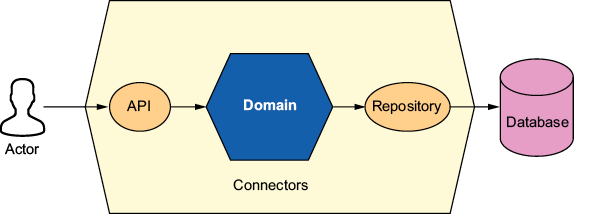
\includegraphics[width=0.94\textwidth]{figures/ch10/CH10_F01_Latour.png}

\medskip
\noindent\textbf{图 10.1\quad 包含领域与连接器的架构图}
\end{center}

原因和第 8 章讲过的一样：代表可传输数据的 Go 结构——这里就是生成代码——必须能够独立于其余代码演化。

\subsection{业务层}

第 8 章中，我们曾创建 \texttt{session} 包来容纳业务逻辑。现在请新建 \texttt{internal/habit} 文件夹，在里面定义领域层的 \texttt{Habit} 以及它需要的类型，如代码清单 10.12 所示。除了保留输入数据，我们还想记住习惯的创建时间，并为它分配一个 ID，方便日后查找。这些字段并不属于输入消息；正因为没有复用 API 结构，我们才可以在这里自由添加。

\begin{gocode}[title={代码清单 10.12 \texttt{internal/habit/habit.go}：定义业务类型}]
// ID is the identifier of the Habit.
type ID string

// Name is a short string that represents the name of a Habit.
type Name string

// WeeklyFrequency is the number of times a Habit should happen every week.
type WeeklyFrequency uint

// Habit to track.
type Habit struct {
    ID              ID #1
    Name            Name
    WeeklyFrequency WeeklyFrequency
    CreationTime    time.Time #1
}
\end{gocode}

\begin{codeannotations}
\item 仅供领域内部使用的字段
\end{codeannotations}

即使写起来略显啰唆，为主实体的每个字段创建专门类型通常仍是个好习惯。这样，函数和方法就能接收有明确类型的参数；类型本身既充当文档，也让 API 更清楚。例如，一个函数同时接收名称和 ID，而二者都是字符串时，很容易把顺序弄反。可要是一个参数明确是 \texttt{ID}，另一个明确是 \texttt{Name}，调用者若把名称强制转换成 ID 类型，眼前理应立刻亮起红灯。

\subsubsection{需求：创建一项习惯}

回头看看需求，首先要做的就是创建 \texttt{Habit}。我们在 Protobuf 文档中声明了一些可选值，这意味着缺失时需要替它们补全。第一道问题是：输入校验该由 API 层负责，还是由领域层负责？两种选择都有各自的道理。我们的决定是：将来若服务内部的某项新功能也要创建习惯，它会直接调用领域层；而我们希望 \texttt{NewHabit} 无论从哪里调用，都只返回有效实体。不能指望 API 层每次都恰好送来领域所需的一切。

\begin{tipbox}{提示}
若你所处的场景更适合在 API 层做校验，可以使用现成库。例如 \url{https://github.com/go-playground/validator} 的 \texttt{validator} 包，只需添加少量标签便能完成许多校验工作。
\end{tipbox}

输入无效时该怎么办？和 HTTP 一样，gRPC 也使用不同状态码来说明 RPC API 所定义响应的含义，表 10.1 列出了其中几个。端点返回响应时，会把这些状态码放进同时返回的错误里。

\Needspace{12\baselineskip}
\begin{center}
\textbf{表 10.1\quad 部分 gRPC 状态码}

\smallskip
\begin{tabularx}{\textwidth}{@{}>{\ttfamily}l >{\ttfamily}c Y@{}}
\toprule
\normalfont\bfseries 代码 & \normalfont\bfseries 编号 & \bfseries 说明 \\
\midrule
OK & 0 & 这不是错误；操作成功时返回。 \\
INVALID\_ARGUMENT & 3 & 客户端给出了无效参数。 \\
NOT\_FOUND & 5 & 请求的某个实体（例如文件或目录）不存在。 \\
PERMISSION\_DENIED & 7 & 调用方无权执行指定操作。 \\
UNIMPLEMENTED & 12 & 该操作尚未实现，或当前服务不支持、未启用该操作。 \\
INTERNAL & 13 & 处理请求时发生了未明确归类的错误。 \\
\bottomrule
\end{tabularx}
\end{center}

这里只列出了一小部分；完整列表和更深入的解释可在官方文档中找到。运行 \texttt{go doc google.golang.org/grpc/codes} 本应能看到列表——好吧，严格来说并不能，因为 \texttt{go doc} 会限制输出，只打印最前面的几个状态码。要查看全部内容，请运行：

\begin{shellcode}[]
> go doc --all google.golang.org/grpc/codes
\end{shellcode}

记住这些状态码之后，我们知道：任何无效输入都应返回编号 3。
这个编号对应的状态码是 \texttt{INVALID\_ARGUMENT}。
业务层当然不该负责返回这个编号；那是 API 层的职责。

领域层甚至不知道我们正在实现 gRPC 服务器，但 API 层又需要知道领域内部究竟发生了什么。正好可以用类型化错误解决。

\subsubsection{使用类型化错误校验}

在 \texttt{habit} 包中新建专门承载这段业务逻辑的 \texttt{create.go}，先实现 \texttt{validateAndCompleteHabit}，如代码清单 10.13 所示。它要检查名称是否为空；频率为空时设为 \texttt{1}；还要补齐两个内部字段。严格说来，这也可以拆成两个函数：一个负责校验，另一个负责补全。

\begin{gocode}[title={代码清单 10.13 \texttt{internal/habit/create.go}：校验并补全实体}]
// validateAndCompleteHabit fills the habit with values that we want in
// our database.
// Returns InvalidInputError. #1
func validateAndCompleteHabit(h Habit) (Habit, error) {
    // name cannot be empty
    h.Name = Name(strings.TrimSpace(string(h.Name))) #2
    if h.Name == "" {
        return Habit{}, InvalidInputError{ #3
            field: "name", reason: "cannot be empty"}
    }

    if h.WeeklyFrequency == 0 {
        h.WeeklyFrequency = 1 #4
    }

    if h.ID == "" {
        h.ID = ID(uuid.NewString()) #5
    }

    if h.CreationTime.Equal(time.Time{}) {
        h.CreationTime = time.Now()
    }

    return h, nil
}
\end{gocode}

\begin{codeannotations}
\item 告诉读者这个函数可能返回什么
\item 一整行空格同样无效
\item 返回结构化错误
\item 默认值为 1
\item 生成新的唯一 ID
\end{codeannotations}

接下来，在 \texttt{habit} 包中新建 \texttt{errors.go}，定义这个类型化错误。

\begin{gocode}[title={代码清单 10.14 \texttt{errors.go}：表示无效输入的类型化错误}]
// InvalidInputError is returned when user-input data is invalid.
type InvalidInputError struct {
    field  string
    reason string #1
}

// Error implements error.
func (e InvalidInputError) Error() string {
    return fmt.Sprintf("invalid input in field %s: %s", e.field, e.reason)
}
\end{gocode}

\begin{codeannotations}
\item 简要说明给定值为何无效
\end{codeannotations}

我们也可以把字段收到的实际值暴露出来。出错时知道服务器究竟收到了什么，非常有用——它和我们\emph{以为}自己发出的内容不一致的次数，往往多得不愿承认。不过，这个错误会被写入日志并到处复制；恶意用户完全可以送来数 GB 的数据，把系统拖垮。限制请求大小、截断日志等办法都能防范这种问题，但现在先简单一点：不要把字段值记进日志。

\subsubsection{测试校验逻辑}

已经可以为 \texttt{validateAndCompleteHabit} 写一个简单的单元测试了。一个依赖都不用 mock——多么令人愉快！

写测试时，我们发现每个测试用例的断言都很不一样，于是为它们分别编写了具名函数。你可以写多个彼此独立的 \texttt{TestXxx}，也可以像下面这样，用明确的名称把它们归入同一个测试。

\begin{gocode}[title={代码清单 10.15 \texttt{create\_internal\_test.go}：测试 \texttt{validateAndCompleteHabit}}]
func Test_validateAndFillDetails(t *testing.T) {
    t.Parallel()

    t.Run("Full", testValidateAndFillDetailsFull)
    t.Run("Partial", testValidateAndFillDetailsPartial)
    t.Run("SpaceName", testValidateAndFillDetailsSpaceName)
}
\end{gocode}

第一个函数 \texttt{testValidateAndFillDetailsFull} 检查：如果习惯本来就完整，任何内容都不应改变。

\begin{gocode}[]
func testValidateAndFillDetailsFull(t *testing.T) {
    t.Parallel()

    h := Habit{/* all fields are filled */}

    got, err := validateAndCompleteHabit(h)
    require.NoError(t, err)
    assert.Equal(t, h, got)
}
\end{gocode}

第二个函数检查：如果习惯信息不完整，ID 和创建时间应当得到补全，其余字段保持不变。每次运行测试得到的值都不同，因此这里只能用 \texttt{NotEmpty} 确认这些字段至少不是空的。若想检查得更严谨，可以用正则表达式确认 ID 符合预期格式，并检查时间是否落在过去一秒左右的范围内。

\begin{gocode}[]
func testValidateAndFillDetailsPartial(t *testing.T) {
    t.Parallel()

    h := Habit{/* only Name and Freq */}

    got, err := validateAndCompleteHabit(h)
    require.NoError(t, err)
    assert.Equal(t, h.Name, got.Name)
    assert.Equal(t, h.WeeklyFrequency, got.WeeklyFrequency)
    assert.NotEmpty(t, got.ID)
    assert.NotEmpty(t, got.CreationTime)
}
\end{gocode}

然后检查名称。若只发送空格，应当得到 \texttt{InvalidInputError}。当前仍处于开发早期，错误的具体内容还可能变化，所以暂时只关注类型。

\begin{gocode}[]
func testValidateAndFillDetailsSpaceName(t *testing.T) {
    t.Parallel()

    h := Habit{Name: "    "}

    _, err := validateAndCompleteHabit(h)
    assert.ErrorAs(t, err, &InvalidInputError{})
}
\end{gocode}

很好。运行测试，确认你对覆盖率感到满意。

现在来真正调用端点。业务层（也就是领域层）的 \texttt{Create} 函数会补全习惯，并准备把它保存到数据存储中。

\begin{gocode}[title={代码清单 10.16 \texttt{create.go}：创建习惯的业务函数}]
// Create validates the Habit, saves it and returns it.
func Create(_ context.Context, h Habit) (Habit, error) {
    h, err := validateAndCompleteHabit(h)
    if err != nil {
        return Habit{}, err #1
    }

    // Need to add the habit to data storage...

    return h, nil
}
\end{gocode}

\begin{codeannotations}
\item 若想补充上下文，也可以在这里包装错误
\end{codeannotations}

你已经可以为它写一个黑盒测试，至少可以先搭出测试结构。我们把 \texttt{context} 作为第一个参数，却一直没有使用。为什么？答案其实很简单，10.6 节会完整解释。现在只需提供一个 \texttt{context.Context} 变量；在 Go 中，它几乎总被命名为 \texttt{ctx}。

\subsection{API 层}

领域层的校验逻辑已经实现，现在回到服务器包，更新服务器结构上的 \texttt{CreateHabit} 方法，如代码清单 10.17 所示。这里属于 gRPC 层：我们把 API 专用签名转换成领域对象，调用领域函数，再把响应转换回 API 专用类型。

\begin{gocode}[title={代码清单 10.17 \texttt{create.go}：API 层}]
// CreateHabit is the endpoint that registers a habit.
func (s *Server) CreateHabit(ctx context.Context,
    request *api.CreateHabitRequest) (*api.CreateHabitResponse, error) {
    var freq uint #1
    if request.WeeklyFrequency != nil {
        freq = uint(*request.WeeklyFrequency)
    }

    h := habit.Habit{
        Name:            habit.Name(request.Name),
        WeeklyFrequency: habit.WeeklyFrequency(freq),
    }

    createdHabit, err := habit.Create(ctx, h)
    if err != nil {
        ...
    }

    s.lgr.Logf("Habit %s successfully registered", createdHabit.ID)

    return &api.CreateHabitResponse{
        Habit: &api.Habit{
            Id:              string(createdHabit.ID),
            Name:            string(createdHabit.Name),
            WeeklyFrequency: int32(createdHabit.WeeklyFrequency),
        },
    }, nil #2
}
\end{gocode}

\begin{codeannotations}
\item 先以默认值 0 初始化
\item 不必返回 \texttt{status.Error(codes.OK, "everything went fine")}
\end{codeannotations}

如果习惯频率的默认值想设为 \texttt{1}，为什么字段缺失时却让 \texttt{freq} 保持为 \texttt{0}——也就是使用 Go 的零值？因为我们把这个默认值视为业务需求，而不是 API 定义。这项决定可以争论，只能结合具体场景判断。设想一下：若从 API 层以外的地方调用领域方法并传入空频率，你希望发生什么？照那个预期去设计即可。

领域层返回的错误该怎样处理？我们已经保证，输入不合法所引发的错误具有特定类型。可以用 \texttt{errors.As} 把它转换为 \texttt{InvalidInputError}，据此判断是否返回编号 3。说实话，这里也可以使用 \texttt{errors.Is}，因为我们没有读取 \texttt{InvalidInputError} 专属的任何字段或方法；但我们想借此展示 \texttt{As} 的用法。

可要是收到的并非 \texttt{InvalidInputError} 呢？毕竟，端点逻辑未来还要访问数据库；数据库调用完全可能出错，而且与输入消息校验无关。

实现 gRPC 端点时，可以记住一条经验法则：每条 \texttt{return} 语句要么返回 \texttt{nil} 错误，要么返回由 \texttt{status.Error}（或 \texttt{Errorf}）构造的错误。

\texttt{status} 包就在 \texttt{codes} 包旁边，导入路径是 \path{google.golang.org/grpc/status}。拿不准该用哪个错误码时，默认选择 \texttt{codes.Internal}，如下所示。

\begin{gocode}[title={代码清单 10.18 \texttt{create.go}：处理错误}]
got, err := habit.Create(ctx, h)
if err != nil {
    var invalidErr habit.InvalidInputError
    if errors.As(err, &invalidErr) {
        return nil, status.Error(codes.InvalidArgument, invalidErr.Error())
    }
    // other error
    return nil, status.Errorf(codes.Internal, "cannot save habit %v: %s",
        h, err.Error())
}
\end{gocode}

当服务拥有多个端点以后，检查错误并输出恰当状态码的逻辑可以抽成一个函数，例如 \texttt{toAPIErrorf(err error, format string, args ...any)}。真正需要时，尽管动手实现。

现在该手动测试服务器了。第 8 章调用服务时使用的 \texttt{curl} 只能发 HTTP 请求，不过它有个表亲 \texttt{grpcurl}，干的是同一类工作。\texttt{grpcurl} 也有不少替代品，很多还带图形界面；但就我们而言，它最顺手。若你偏爱漂亮的 GUI，Postman 也支持 gRPC，并从版本 10 起便能向服务器发送 Protobuf 消息。

先运行 \texttt{go run cmd/habits-server/main.go} 启动服务器，再用下面的命令安装 \texttt{grpcurl}：

\begin{shellcode}[]
> go install github.com/fullstorydev/grpcurl/cmd/grpcurl@latest
\end{shellcode}

现在可以用它向服务器发送请求。\texttt{curl} 与 \texttt{grpcurl} 有个重要区别：对 \texttt{curl} 而言，消息只是普通 JSON 文档；对 \texttt{grpcurl} 而言，我们必须提供有效的 Protobuf 实体。还记得本章开头吗？Protocol Buffers 的字段带有编号，这意味着通过 \texttt{grpcurl} 发送的消息必须按正确结构书写，字段也要落在正确位置。这里有两种选择：把 Protobuf 定义交给 \texttt{grpcurl}，或者让它向服务器询问定义。后一种方式称为\emph{反射}（reflection），这里不用。反射会给服务器带来少量额外开销，而我们通常不希望把它带进生产环境。

要告诉 \texttt{grpcurl} 怎样组织请求、怎样理解响应，只需通过 \texttt{-proto} 参数传入 \texttt{.proto} 文件。这里给它 \texttt{service.proto}，因为端点都定义在其中。某些文件还会导入其他文件，因此要用 \texttt{-import-path} 指定这些相对引用的根目录。最后，还得告诉工具目标端点；它是请求的最后一个参数，形式为 \texttt{\{package\}.\{service\}/\{endpoint\}}。可以运行下面这条命令：

\begin{shellcode}[]
> grpcurl \
    -import-path /.../learngo-pockets/habits/api/proto/ \ #1
    -proto service.proto \ #2
    -plaintext -d '{"name":"clean the kitchen"}' \ #3
    localhost:28710 \ #4
    habits.Habits/CreateHabit #5
\end{shellcode}

\begin{codeannotations}
\item Proto 目录的绝对路径
\item 声明服务的文件
\item 以 JSON 格式提供请求
\item 服务器运行所在的主机与端口
\item 目标端点
\end{codeannotations}

一切顺利的话，应当会收到服务器返回的响应，并以 JSON 格式显示。里面有 ID 字段吗？每周频率设置好了吗？你也试过给习惯传一个“无效”名称了吗？

再看看服务器输出——每收到一个请求，它都应该记录一条日志。若测试结果令人满意，就该让端点做点比记录日志更多的事情了！

\subsection{保存数据}

服务对客户端声称自己能创建习惯，却根本没有把它们存下来。这个问题得解决。保存数据有多种选择，最常见的是数据库；附录 G 展示了怎样连接数据库。

\subsubsection{仓库包}

第一个版本可以沿用第 8 章保存游戏时使用的内存仓库，把它放在 \texttt{internal/repository} 包里。它同样无法扩展，也很可能不够稳定，但能让我们迅速拿到可用结果；对概念验证而言已经足够。

编写一个 \texttt{HabitRepository} 结构和用于构造、初始化内部数据映射的 \texttt{New} 函数。和服务器包的 \texttt{New} 一样，这里也要注入一个 \texttt{Logger}。眼下 \texttt{HabitRepository} 只需要一个 \texttt{Add} 方法，不过很快还会添加 \texttt{FindAll}，用来返回数据库里的全部内容。

如果你一路跟着我们走完了前九章，现在应当已经能够独立创建这个包，暴露正确的函数、结构和方法，当然也会补上测试。别忘了加一把互斥锁，在读写仓库存储时保护数据：

\begin{shellcode}[]
> go doc
package repository // import "learngo-pockets/habits/internal/repository"

Package repository accesses the habits data.

type Error string
type Logger {...}
type HabitRepository struct{ ... }
    func New(lgr Logger) *HabitRepository

> go doc HabitRepository
package repository // import "."

type HabitRepository struct {
        // Has unexported fields.
}
    HabitRepository holds all the current habits.

func New(lgr Logger) *HabitRepository
func (hr *HabitRepository) Add(_ context.Context, habit habit.Habit) error
func (hr *HabitRepository) FindAll(_ context.Context) ([]habit.Habit, error)
\end{shellcode}

我们为每个方法都预留了 \texttt{context.Context} 参数。这样，将来把内存仓库换成真实数据库时，只要客户端中断调用，就能借助上下文停止继续查找数据。需要参考代码的话，本书仓库在 \url{https://mng.bz/nRj2} 提供了一个示例。

\subsubsection{依赖注入}

我们其实没有认真测试这个 \texttt{repository} 包。主要原因是，它所做的不过是向 \texttt{map} 写入数据，以及列出 \texttt{map} 里的全部值。接下来可以把 \texttt{Add} 调用放进领域函数。

服务器包已经完成 API 到领域的连接，但右侧的调用链还缺一截。为补上它，服务器需要持有 \texttt{Repository} 连接器的实例，而领域层的 \texttt{Create} 函数则要接收一个只含 \texttt{Add} 的小接口。

先把仓库依赖注入服务器，如代码清单 10.19 所示。可是，为什么不直接在服务器内部调用 \texttt{repository.New()}，非要放到 \texttt{main} 函数里？稍后会看到，这能让测试简单得多，不必依赖某个写死的实现。这正是 Go 轻量接口最出色的用途之一。这里使用接口，就是为了让服务器测试能够使用 mock。

\begin{gocode}[title={代码清单 10.19 \texttt{server.go}：为服务器添加仓库连接器}]
// Server is the implementation of the grpc server.
type Server struct {
    api.UnimplementedHabitsServer
    db  Repository
    lgr Logger
}

type Repository interface { #1
    Add(ctx context.Context, habit habit.Habit) error
    FindAll(ctx context.Context) ([]habit.Habit, error)
}

// New returns a Server that can Listen.
func New(repo Repository, lgr Logger) *Server {
    return &Server{
        db:  repo,
        lgr: lgr,
    }
}
\end{gocode}

\begin{codeannotations}
\item 只声明当前所需的最小接口
\end{codeannotations}

第一步，更新 \texttt{main} 函数，使它符合 \texttt{New} 的新签名。我们要传入一个实现该接口的值，例如 \texttt{repository.New(...)} 的返回结果。

第二步，领域层的 \texttt{Create} 端点也要接收一个接口参数，如代码清单 10.20 所示。这既方便 stub 和 mock，也能缩小问题范围。接口只有一个 \texttt{Add} 方法，就能保证 \texttt{Create} 无法偷偷调用未来添加的其他方法，把逻辑搅乱。假设你从日志里发现，\texttt{FindEverything} 调用正在拖慢服务性能。看一眼这个接口，就知道罪魁祸首绝不可能是 \texttt{Create}，于是可以继续往别处查。

\begin{gocode}[title={代码清单 10.20 \texttt{create.go}：在逻辑函数中调用仓库}]
type habitCreator interface {
    Add(ctx context.Context, habit Habit) error
}

// Create adds a habit into the DB.
func Create(ctx context.Context, db habitCreator, h Habit) (Habit, error) {
    h, err := validateAndCompleteHabit(h)
    if err != nil {
        return Habit{}, err
    }

    err = db.Add(ctx, h)
    if err != nil {
        return Habit{}, fmt.Errorf("cannot save habit: %w", err)
    }

    return h, nil
}
\end{gocode}

从日志里能看到调用一路抵达数据库了吗？我们来写几个测试，确保错误都被正确捕获。先像第 6 章那样，用一个简单存根实现 \texttt{habitCreator} 接口。

可是，怎样更新 \texttt{Create} 的测试，才能确认 \texttt{Add} 确实得到了调用？下一节就来解决。

\section{使用生成的 mock 做单元测试}

前几章已经展示过：接口足够小、逻辑足够简单时，可以亲手编写存根。不过，也有一些库能读取接口，自动替你生成 mock。

\begin{infobox}{定义：stub 与 mock}
在测试中利用接口，最常见的两种方式就是 stub 和 mock。\emph{使用存根}（stubbing）是编写一个实现接口、返回硬编码值的结构，用来验证依赖返回这个值或那个值时，代码会怎样表现。\emph{使用模拟对象}（mocking）则更进一步：它还会检查每项依赖被调用了多少次，以及调用时传入的参数是否正确。
\end{infobox}

\subsection{生成 mock}

较为知名的库包括 \texttt{mockgen}、\texttt{mockify} 和 \texttt{minimock}。它们背后的设计取舍各不相同，选自己喜欢的即可。本例选择 \texttt{minimock}，因为它生成的模拟函数带有明确类型的参数。运行下面的命令安装：

\begin{shellcode}[]
> go install github.com/gojuno/minimock/v3/cmd/minimock@latest
\end{shellcode}

既然 mock 是生成的，这正是使用 \texttt{go:generate} 语法的好机会。选一个接口，例如 \texttt{habitCreator}，在接口声明之前加入下面一行：

\begin{gocode}[]
//go:generate minimock -i habitCreator -s "_mock.go" -o "mocks"
type habitCreator interface {
    ...
}
\end{gocode}

这条指令要求 \texttt{minimock} 为接口（\texttt{-i}）\texttt{habitCreator} 生成 mock，生成文件使用指定后缀（\texttt{-s}），并写入指定输出文件夹（\texttt{-o}）。继续之前需要先创建该文件夹；从模块根目录看，它就是 \texttt{internal/habit/mocks}。在你喜欢的终端里进入 \texttt{habit} 包，然后运行：

\begin{shellcode}[]
> go generate .
\end{shellcode}

也可以留在模块根目录，一次运行项目中的全部生成命令：

\begin{shellcode}[]
> go generate ./...
\end{shellcode}

此时，\texttt{mocks} 文件夹里会出现一个新文件。用 \texttt{go doc} 看看它提供了什么：

\begin{shellcode}[]
> go doc internal/habit/mocks
package mocks // import "learngo-pockets/habits/internal/habit/mocks"

type HabitCreatorMock struct{ ... }
    func NewHabitCreatorMock(t minimock.Tester) *HabitCreatorMock
type HabitCreatorMockAddExpectation struct{ ... }
type HabitCreatorMockAddParams struct{ ... }
type HabitCreatorMockAddResults struct{ ... }
\end{shellcode}

\subsection{使用 mock}

\texttt{Create} 的黑盒测试现在编译不过了，我们来修好它。首先需要增加两个导入。第一个一看就懂，第二个则值得稍作解释。

\begin{gocode}[]
import (
    // ...
    "learngo-pockets/habits/internal/habit/mocks"
    "github.com/gojuno/minimock/v3"
)
\end{gocode}

第一个导入用于访问刚刚生成的 mock。第二个导入的则是 \texttt{minimock} 库本身。

要是观察得格外仔细，你会发现第二条导入路径以 \texttt{/v3} 结尾。难道我们真的导入了一个名为 \texttt{v3} 的包？那可真是个古怪的包名。

\begin{infobox}{Go 模块的版本管理}
有时，模块要经历大幅改动，新版本无法再与旧版本兼容。只要向后兼容性中断，主版本号就必须变化；与此同时，\texttt{go.mod} 也要反映这个版本。例如，\texttt{minimock} 的 \texttt{go.mod} 第一行就是 \texttt{module github.com/gojuno/minimock/v3}。

希望使用 \texttt{minimock} 或其他带主版本号模块的用户，必须记得在导入路径中、紧接模块名之后写出所需版本。例如：\texttt{import "github.com/jackc/pgx/v5"} 和 \texttt{import "github.com/jackc/pgx/v5/pgxpool"}。但调用这些包中定义的函数或类型时，要忽略路径里的 \texttt{/v5}，仍然写成 \texttt{pgx.Connect(...)} 或 \texttt{pgxpool.New(...)}。
\end{infobox}

之所以还要直接使用 \texttt{minimock} 库，是因为生成代码本身没有提供足够的工具。生成的 \texttt{mocks} 包会暴露 \texttt{NewHabitCreatorMock(...)}，返回我们需要的 \texttt{HabitCreatorMock}——也就是 \texttt{habitCreator} 接口的一种实现。但这个函数需要一个 \texttt{minimock.Tester} 类型的参数。别担心，不必再导入第三个包。

现在，可以为每个测试用例定义一个构建 mock 的函数。它接收控制器，返回所需接口 \texttt{habitCreator} 的模拟实例，如代码清单 10.21 所示。测试用例结构将新增一个函数类型字段。老实说，若你查看本书仓库中包含错误用例的完整测试（\url{https://mng.bz/8OYz}），会发现把它写成两个独立函数更容易读；不过，我们想借此展示：把函数放进测试用例结构体的字段里，也能让生活轻松不少。

控制器在测试开始时创建，所有测试用例都可以共用。此外，只要 \texttt{minimock} 版本足够新（v3.3.0 或更高），它就会在测试结束时自动注册检查，确保每次预期调用都确实发生。对于正常用例，也就是 happy path，mock 应接收之前用变量 \texttt{h} 声明的输入习惯，并返回 \texttt{nil} 错误。

\begin{gocode}[title={代码清单 10.21 \texttt{create\_test.go}：为每个测试用例添加 mock 构造函数}]
tests := map[string]struct {
    db func(
        *minimock.Controller) *mocks.HabitCreatorMock
    expectedErr error
}{
    "nominal": {
        db: func(ctl *minimock.Controller) *mocks.HabitCreatorMock {
            db := mocks.NewHabitCreatorMock(ctl)
            db.AddMock.Expect(ctx, h).Return(nil) #1
            return db
        },
        expectedErr: nil,
    },
}
\end{gocode}

\begin{codeannotations}
\item 登记预期调用
\end{codeannotations}

最后，把它接入 \texttt{TestCreate} 函数。

\begin{gocode}[title={代码清单 10.22 \texttt{create\_test.go}：在测试中使用 mock}]
t.Run(name, func(t *testing.T) {
    t.Parallel()

    ctrl := minimock.NewController(t)
    defer ctrl.Finish() #1

    db := tt.db(ctrl)

    got, err := habit.Create(ctx, db, h)
    assert.ErrorIs(t, err, tt.expectedErr)
    if tt.expectedErr == nil {
        assert.Equal(t, h.Name, got.Name)
    }
})
\end{gocode}

\begin{codeannotations}
\item \texttt{minimock} 3.3.0 及更高版本已不再需要这一行
\end{codeannotations}

代码能够运行，测试也会通过。不妨先提交一次，留住这个正常状态，然后再随意折腾 mock。比如，把 \texttt{Add} 调用注释掉会怎样？测试应该会明确告诉你。

你还可以阅读 \texttt{mocks} 包以及 \texttt{minimock} 工具的文档，找到最合自己口味的写法。对于这种 CRUD（创建、读取、更新、删除）服务，还有一种测试方式尤其合适：集成测试。

\section{集成测试}

单元测试聚焦于一个函数，集成测试则通过完整场景检查整个服务的行为。下面是这个服务可以采用的两个场景。

\begin{description}
  \item[场景 1：添加并列出]
  添加一项习惯：每周去森林散步三次；
  添加一项习惯：每周给植物浇水两次；
  列出习惯，检查返回的两项习惯；
  添加一项习惯：每周读书五次；
  再次列出习惯，检查返回的三项习惯。

  \item[场景 2：添加并删除]
  添加一项习惯：每周去森林散步三次；
  列出习惯，检查返回的一项习惯；
  添加一项没有名称的习惯，预期得到编号 3 的错误；
  添加一项习惯：每周给植物浇水两次；
  列出习惯，检查返回的两项习惯；
  删除第一项习惯；
  再次列出习惯，检查第二项仍然存在。
\end{description}

场景当然还可以有很多。有些人会把它们与 API 测试交织在一起；另一些人则会把业务流程测试，与各端点错误用例的 gRPC 响应测试分开。要验证完整流程，我们首先得能列出已经保存的习惯。实现之后，就可以编写第一个场景了。

\subsection{列出习惯}

添加一个端点需要补几处内容，但做起来应该很快。请按以下步骤进行。

\begin{enumerate}
  \item 更新 Protobuf 文件，加入 \texttt{ListHabits} 端点，如代码清单 10.23 所示。这样一来，已经可以把接口发布给团队其他成员，让他们调用或生成 mock。
\end{enumerate}

\begin{protocode}[title={代码清单 10.23 \texttt{service.proto}：添加列出习惯的端点}]
// Habits is a service for registering and tracking habits.
service Habits {
  // CreateHabit is the endpoint that registers a habit.
  rpc CreateHabit(CreateHabitRequest) returns (CreateHabitResponse);

  // ListHabits is the endpoint that returns all habits.
  rpc ListHabits(ListHabitsRequest) returns (ListHabitsResponse);
}

// ListHabitsRequest is the request to list all the habits saved.
message ListHabitsRequest { #1
}

// ListHabitsResponse is the response with all the saved habits.
message ListHabitsResponse {
  repeated Habit habits = 1; #2
}
\end{protocode}

\begin{codeannotations}
\item 这个请求不含任何参数
\item Protobuf 使用这种方式表示数组
\end{codeannotations}

\begin{enumerate}[resume]
  \item 重新生成对应的 Go 文件：
\end{enumerate}

\begin{shellcode}[]
> go generate ./...
\end{shellcode}

\begin{enumerate}[resume]
  \item 参照 \texttt{internal/habit/create.go} 的模式，在领域层添加逻辑，如代码清单 10.24 所示。别忘了为数据库声明一个小接口、为它生成 mock，并认真测试。不过，测试并不总需要 mock 框架。除了用一个简单函数替代数据库行为，也可以定义一个结构体，保存想要模拟的输出，再让数据库调用直接返回它。
\end{enumerate}

\begin{gocode}[title={代码清单 10.24 \texttt{list\_test.go}：不使用 \texttt{minimock} 测试列表功能}]
// MockList is a mock for FindAll method response.
type MockList struct { #1
    Items []habit.Habit
    Err   error
}

// FindAll is a mock which returns the passed list of items and error.
func (list MockList) FindAll(context.Context) ([]habit.Habit, error) {
    return list.Items, list.Err
}

func TestListHabits(t *testing.T) {
    habits := []habit.Habit{/* ... */}
    dbErr := errors.New("database error")

    tests := map[string]struct {
        db             MockList
        expectedErr    error
        expectedHabits []habit.Habit
    }{
        "empty": {
            db:             MockList{Items: nil, Err: nil}, #2
            expectedErr:    nil,
            expectedHabits: nil,
        },
        "2 items": {
            db:             MockList{Items: habits, Err: nil},
            expectedErr:    nil,
            expectedHabits: habits,
        },
        "error case": {
            db:             MockList{Items: nil, Err: dbErr},
            expectedErr:    dbErr,
            expectedHabits: nil,
        },
    }

    for name, tc := range tests {
        name, tc := name, tc

        t.Run(name, func(t *testing.T) {
            t.Parallel()

            got, err := habit.ListHabits(
                context.Background(), tc.db) #3
            assert.ErrorIs(t, err, tc.expectedErr)
            assert.ElementsMatch(t, tc.expectedHabits, got)
        })
    }
}
\end{gocode}

\begin{codeannotations}
\item 要模拟的数据库调用输出：习惯列表和错误
\item 填入调用 \texttt{FindAll} 时数据库应返回的内容
\item 调用模拟的数据库接口
\end{codeannotations}

\begin{enumerate}[resume]
  \item 若尚未实现，就编写列出所有已保存习惯的仓库函数，如下一段代码所示。仓库应返回确定性的习惯列表，可按固定标准排序，例如习惯的创建时间。
\end{enumerate}

\begin{gocode}[title={代码清单 10.25 \texttt{memory.go}：以确定顺序返回习惯}]
// FindAll returns all habits sorted by creation time.
func (hr *HabitRepository) FindAll(
    _ context.Context) ([]habit.Habit, error) {
    hr.lgr.Logf("Listing habits, sorted by creation time...")

    // Lock the reading and the writing of the habits.
    hr.mutex.Lock()
    defer hr.mutex.Unlock()

    habits := make([]habit.Habit, 0)
    for _, h := range hr.habits {
        habits = append(habits, h)
    }

    // Ensure the output is deterministic by sorting the habits.
    sort.Slice(habits, func(i, j int) bool { #1
        return habits[i].CreationTime.Before(habits[j].CreationTime)
    })

    return habits, nil
}
\end{gocode}

\begin{codeannotations}
\item 就地实现按创建时间为习惯排序的逻辑
\end{codeannotations}

\begin{enumerate}[resume]
  \item 参照 \texttt{internal/server/create.go} 的模式，为服务添加 \texttt{ListHabits} 方法。把生成结构与领域结构之间的转换隔离到单独函数中，并为它编写单元测试。我们认为仓库里没有任何习惯并不算问题，不应返回错误；你也可以作出不同选择。另外请考虑确定性：仓库里若有两个元素，端点是否应当始终按同一顺序返回？确定性非常重要，我们强烈建议尽可能主动保证。确定性端点可比非确定性端点好测多了！
  \item 使用 \texttt{grpcurl} 或类似工具手动测试。
\end{enumerate}

确认新端点如预期工作之后，就可以编写集成测试了。

\subsection{通过 \texttt{go test} 运行集成测试}

我们希望测试穿过服务的每一层，一直抵达服务外部的网络。眼下的数据库只是一个取巧的内存实现，没有必要 mock；等真正换成数据库系统时，要么得 mock，要么得在本地启动一个实例。这个测试会真刀真枪地运行服务，再像普通客户端那样调用它。

\subsubsection{运行服务}

首先创建 \texttt{internal/server/integration\_test.go}，在其中添加 \texttt{TestIntegration}，如代码清单 10.26 所示。集成测试文件可以放在很多地方；因为这里测试的是服务器 API，我们选择让它待在服务器旁边。

第一步，创建并注册一个 gRPC 服务器实例，与 \texttt{main} 函数中已有的逻辑相似。第二步，创建监听器；把空字符串作为地址参数，就等于请它在本机寻找一个空闲端口并使用。第三步，在 goroutine 中运行服务器，让测试余下部分继续执行，并能向它发起调用。当然，无论测试何时结束，都必须把服务器停下来。

若需要编写辅助函数，可以在函数开头调用 \texttt{t.Helper()}。这样，Go 测试套件报告错误时就会略过这一层，把位置指向真正调用辅助函数的测试代码。

\begin{gocode}[title={代码清单 10.26 \texttt{integration\_test.go}：启动服务}]
func TestIntegration(t *testing.T) {
    grpcServ := newServer(t)
    listener, err := net.Listen("tcp", "")
    require.NoError(t, err)

    wg := sync.WaitGroup{}
    wg.Add(1)
    go func() {
        defer wg.Done()
        err = grpcServ.Serve(listener)
        assert.NoError(t, err)
    }()
    defer func() {
        // terminate the GRPC server
        grpcServ.Stop()
        // when that is done, and no error were caught, we can end this test
        wg.Wait() #1
    }()

    // ... scenario follows
}

func newServer(t *testing.T) *grpc.Server {
    t.Helper() #2

    s := server.New(repository.New(t), t) #3

    grpcServer := grpc.NewServer(
        grpc.UnaryInterceptor(timerInterceptor(s.lgr)))
    api.RegisterHabitsServer(grpcServer, s)
    reflection.Register(grpcServer)

    return grpcServer
}
\end{gocode}

\begin{codeannotations}
\item 使用 \texttt{WaitGroup}，确保 goroutine 已经检查过 \texttt{Serve} 返回的错误
\item 打印测试详情时略过这个辅助函数
\item \texttt{t} 拥有 \texttt{Logf} 方法，因此同时实现了 \texttt{server.Logger} 和 \texttt{repository.Logger}
\end{codeannotations}

服务器已经运行，客户端可以登场了。下一步就来处理它。

\subsubsection{创建客户端}

客户端必须知道请求要发往哪个地址，也必须了解服务器的形状——也就是有哪些端点。我们编写一个构造客户端的函数，让它接收服务器地址，如代码清单 10.27 所示。

注意，连接服务器时需要传入凭据。\texttt{grpc} 库体贴地提供了一个函数，可以生成关闭传输层安全协议（Transport Layer Security，TLS）的凭据。通常这么做会造成安全漏洞，不过当前服务器运行在限制非常严格的环境中，我们可以接受不提供真正凭据。请求会经过怎样的网络，决定了你究竟必须使用安全凭据，还是可以借助 \texttt{insecure} 包生成“不安全凭据”。

\begin{gocode}[title={代码清单 10.27 \texttt{integration\_test.go}：创建客户端}]
func TestIntegration(t *testing.T) {
    ...
    // create client
    habitsCli, err := newClient(t, listener.Addr().String())
    require.NoError(t, err)
}

func newClient(t *testing.T, serverAddress string) (api.HabitsClient, error) {
    t.Helper()
    creds := grpc.WithTransportCredentials(
        insecure.NewCredentials(),
    ) #1
    conn, err := grpc.Dial(serverAddress, creds)
    if err != nil {
        return nil, err
    }

    return api.NewHabitsClient(conn), nil
}
\end{gocode}

\begin{codeannotations}
\item \texttt{insecure} 的意思就是“不使用 TLS”
\end{codeannotations}

舞台布置完毕，可以开始跑场景了。

\subsubsection{运行场景}

目前只测试两个端点，可以为它们各写一个正常路径辅助函数。然后，再为 \texttt{CreateHabit} 编写一个错误路径函数；\texttt{ListHabits} 不会返回业务错误，因此不需要。

代码清单 10.28 展示了列出习惯的端点。它是两者中稍棘手的那个，因为返回的 ID 是生成出来的，每次运行值都会变化。因此，先确认 \texttt{Id} 字段已经填好，再把它覆盖掉。

\begin{gocode}[title={代码清单 10.28 \texttt{integration\_test.go}：列出并核对 \texttt{Habit}}]
func listHabitsMatches(
    t *testing.T, habitsCli api.HabitsClient, expected []*api.Habit) {
    list, err := habitsCli.ListHabits(
        context.Background(), &api.ListHabitsRequest{})
    require.NoError(t, err)

    for i := range list.Habits {
        assert.NotEqual(t, "", list.Habits[i].Id)
        list.Habits[i].Id = "" #1
    }
    assert.Equal(t, expected, list.Habits) #2
}
\end{gocode}

\begin{codeannotations}
\item 这个字段的值是随机生成的；这里只确认它不为空
\item 非确定性端点应使用 \texttt{ElementsMatch}，确定性端点则使用 \texttt{Equal}
\end{codeannotations}

也可以考虑让集成测试围绕一个结构体组织：结构体把客户端保存为字段，并通过方法包装客户端调用，使测试更容易阅读。我们只使用了函数，但所有函数都以相同的两个参数开头，写多了会非常啰唆——这通常正是该重构的信号。有了这类辅助函数，场景代码可以读得相当顺畅。

\begin{gocode}[title={代码清单 10.29 \texttt{integration\_test.go}：用代码表达场景}]
// add 2 habits
addHabit(t, habitsCli, nil, "walk in the forest")
addHabit(t, habitsCli, ptr(3), "read a few pages")
addHabitWithError(t, habitsCli, 5, "        ", codes.InvalidArgument)

// check that the 2 habits are present
listHabitsMatches(t, habitsCli, []*api.Habit{...})

// ...

func ptr(i int32) *int32 {
    return &i
}

func addHabit(t *testing.T, habitsCli api.HabitsClient,
    freq *int32, name string) {
    _, err := habitsCli.CreateHabit(context.Background(),
        &api.CreateHabitRequest{
            Name:            name,
            WeeklyFrequency: freq,
        })
    require.NoError(t, err)
}
\end{gocode}

一定要让不同场景彼此隔离，这样它们才能并行运行。甚至可以为每个集成场景并行启动一个独立服务器实例。你还可以趁机玩玩并发：并发调用大量 \texttt{Add}，检查性能表现。

\subsubsection{使用 \texttt{testing.Short} 只运行轻量测试}

到目前为止，这个测试看起来和写过的其他单元测试没多大区别，只是名字叫“集成测试”。但有时集成测试会很重：它们穿过大量功能和用例，包含一些基准测试，或者执行负载与性能测试。此类测试往往耗时很久，不建议每次都放进持续集成（continuous integration，CI）流水线，以免拖慢交付。例如，可以要求拉取请求只运行“轻量”测试，而打标签和构建镜像时才运行“重量”测试。

\texttt{go test ./...} 接受 \texttt{-short} 标志。命令行带上这个标志，会改变 \texttt{testing.Short()} 的返回值；任何测试都能调用这个函数。先在 \texttt{TestIntegration} 开头检查该标志：

\begin{gocode}[]
func TestIntegration(t *testing.T) {
    // Skip this test when running lightweight suites
    if testing.Short() {
        t.Skip()
    }

    grpcServ := newServer(t)
    // ...
}
\end{gocode}

现在看看 \texttt{go test -v ./...} 的输出。\texttt{-v} 会启用详细模式，列出调用的每个测试函数；输出中应当出现 \texttt{TestIntegration}：

\begin{shellcode}[]
> go test -v ./...
...
ok      learngo-pockets/habits/internal/habit    1.004s
=== RUN   TestIntegration
    create.go:17: Create request received: name:"walk in the forest"
...
--- PASS: TestIntegration (0.00s)
...
\end{shellcode}

再试一次，这回加上 \texttt{short} 标志。下面的输出应明确表明 \texttt{TestIntegration} 被跳过了：

\begin{shellcode}[]
> go test -v -short ./...
...
ok      learngo-pockets/habits/internal/habit    1.004s
=== RUN   TestIntegration
    integration_test.go:23:
--- SKIP: TestIntegration (0.00s)
...
\end{shellcode}

至此，我们已经能在 CI 流水线里只运行轻量测试。编写成本更高、资源消耗更大的测试时，请检查 \texttt{-short} 标志；它的出现表示我们想尽快拿到结果。

到目前为止，服务一直使用我们信任的内存数据库。如果它不可用，服务器会遇到严重问题，因为服务器和数据库本来就是同一个程序的一部分。但现实中，数据库大多是远程实体，可能因网络故障、外部负载或其他恼人的 bug 而表现失常。更糟的是，万一我们自己的查询把数据库打崩了呢？数据库返回错误的情况已经处理，可它要是根本不回答呢？我们该等多久，才承认事情确实不对劲？

\section{充分利用上下文}

依赖远程服务时，一个常见的良好实践是：只允许被调用方在规定时间内给出响应。表达时间限制有两种方式。可以给出超时时长（timeout），就像《碟中谍》里的“本消息将在 5 秒后自毁”；也可以给出截止时间（deadline），例如“你可以做到星期五上午 11 点”。该选哪一种取决于具体活动，不过调用远程网络实体时，前者远比后者常见。

\subsection{上下文是什么？}

本章前面提到过 \texttt{Context}，却一直没有真正定义它。现在运行 \texttt{go doc context.Context} 看看。文档告诉我们，\texttt{Context} 用于跨越 API 边界携带截止时间、取消信号和值；它是一个包含以下方法的接口：

\begin{itemize}
  \item \texttt{Value(key any) any}
  \item \texttt{Deadline() (deadline time.Time, ok bool)}
  \item \texttt{Done() <-chan struct\{\}}
  \item \texttt{Err() error}
\end{itemize}

继续之前要特别强调：\texttt{context.Context} 虽然是接口，却属于极少数你几乎永远不该亲自实现的接口。

\texttt{Context} 的 \texttt{Value} 方法用于满足“跨 API 边界携带值”这项需求。你当然可以把 \texttt{Context} 看成键值存储，但我们强烈建议别这么想。若把重要值塞进 \texttt{Context}，不同函数究竟需要哪些输入，就再也无法从签名上一眼看清。上下文只适合传递非关键数据，例如监控标识符或请求标识符；业务值不应通过 \texttt{Context} 传递。若你正考虑这么做，最好另寻方案。10.6.3 节会给出一个使用 \texttt{Context} 存储能力的例子。

\texttt{Deadline} 方法返回 \texttt{Context} 是否设置了截止时间，以及具体截止到何时。到了那个时刻，谁来询问，这个 \texttt{Context} 都会回答：“我已经过期了。”

\texttt{Done} 方法返回一个通道；\texttt{Context} 走到生命尽头时，这个通道会被关闭。调用 \texttt{Done()} 比拿 \texttt{Deadline()} 与 \texttt{time.Now()} 比较更简单，因此通常都会选择前者。

最后，\texttt{Err} 方法会返回一个错误，说明 \texttt{Done} 所返回的通道为何关闭；若通道尚未关闭，则返回 \texttt{nil}。知道它是什么之后，来看看怎样创建 \texttt{Context}。

\subsection{创建上下文}

Go 的 \texttt{context} 包提供了若干创建 \texttt{Context} 的函数，大致分成两类：一类根据父 \texttt{Context} 创建子上下文，另一类则凭空创建一个上下文。

后一类只有 \texttt{context.Background()} 和 \texttt{context.TODO()}。我们建议始终在 \texttt{main} 函数中创建应用的 \texttt{Context}，再把它传给所有可能需要的依赖。使用 \texttt{Background} 创建，并尽量避免调用 \texttt{TODO}。总体而言，一个应用应当只有一个父 \texttt{Context}。

拿到一个 \texttt{Context} 以后，就能创建它的子上下文。子上下文可以有多种形态，主要区别在于怎样设置 \texttt{Deadline}。调用 \texttt{WithDeadline} 可以指定一个确切时间点，届时子上下文会被取消；若想指定 \texttt{Context} 应该“活”多久，则调用 \texttt{WithTimeout}。远程服务调用中，第二种做法远为常见。

不过，大多数时候，函数会把 \texttt{Context} 作为参数接收。有一条不成文的约定：\texttt{Context} 总是函数调用的第一个参数；就像错误通常命名为 \texttt{err}，上下文也几乎总叫 \texttt{ctx}。函数既然已经收到一个 \texttt{Context}，就不该再用 \texttt{Background()} 或 \texttt{TODO()} 另起炉灶。观察 gRPC 生成代码会发现，所有端点签名都以传入的 \texttt{Context} 开头——该用的正是它。

每次都把 \texttt{Context} 作为参数传递，看起来也许有些重复；但请务必忍住，别为了省事用组合把 \texttt{Context} 存进结构体字段。

\subsection{使用上下文}

究竟在什么场景下该创建子 \texttt{Context}？为什么不直接传父上下文？毕竟父上下文自己也可能带有截止时间。答案关系到良好的编码习惯，以及对每次跨网络调用进行精确控制。假设一个服务为了回答请求，需要再调用另外两个服务；若其中一个迟迟不返回，我们希望能清楚知道究竟是哪一个。要做到这一点，每次远程调用都必须使用自己的 \texttt{Context} 和自己的截止时间。根据应用性质，超时时长可以短至 10 ms，也可以长达数天。不要卡得过分严苛，还要把网络延迟算进去。

拿数据库举例。假设我们要确保 \texttt{Create} 端点中的仓库调用不会耗时过久。代码清单 10.30 展示了做法：调用仓库之前，创建一个超时时间为 100 ms 的 \texttt{Context}。

\begin{gocode}[title={代码清单 10.30 \texttt{create.go}：用 \texttt{context} 包住数据库调用}]
// Create adds a habit into the DB.
func Create(ctx context.Context, db habitCreator, h Habit) (Habit, error) {
    h, err := validateAndCompleteHabit(h)
    if err != nil {
        return Habit{}, err
    }

    dbCtx, cancel := context.WithTimeout(
        ctx, 100*time.Millisecond) #1
    defer cancel() #2
    err = db.Add(dbCtx, h) #3
    if err != nil {
        return Habit{}, fmt.Errorf("cannot save habit: %w", err)
    }

    return h, nil
}
\end{gocode}

\begin{codeannotations}
\item 始终复用父上下文
\item 确保函数结束时清理资源
\item 别忘了真正使用新上下文
\end{codeannotations}

运行之后，一切正常，但这项行为还没有测试——而我们理应测试。情况甚至比“没测试”更糟：它直接把现有测试弄坏了！还记得吗，我们使用的是 mock，而 mock 对自己的预期非常严格。此前的测试没怎么在意 \texttt{Context}，毕竟我们也从未动过它。现在，\texttt{Create} 端点调用 \texttt{Add} 时使用的已经不再是那个 \texttt{Background} 上下文。测试必须更新，可要提供一模一样的 \texttt{Context}，就得精确知道截止时间是什么时候，才能写出正确预期。

许多 mock 库迟早都会碰上这个问题。\texttt{minimock} 的选择是暴露一个 \texttt{minimock.AnyContext} 变量，让它匹配任意 \texttt{context.Context}。另一些库走得更远，提供 \texttt{mock.Anything}，可作为任意输入参数的通配符。我们只需要放宽 \texttt{Context}，因此用前一种就够了。

\begin{gocode}[title={代码清单 10.31 \texttt{create\_test.go}：模拟子 \texttt{context}}]
func TestCreate(t *testing.T) {
    // ...
    "nominal": {
        db: func(ctl *minimock.Controller) *mocks.HabitCreatorMock {
            db := mocks.NewHabitCreatorMock(ctl)
            db.AddMock.Expect(minimock.AnyContext, h). #1
                Return(nil)
            return db
        },
        expectedErr: nil,
    },
    "error case": {
        db: func(ctl *minimock.Controller) *mocks.HabitCreatorMock {
            db := mocks.NewHabitCreatorMock(ctl)
            db.AddMock.Expect(minimock.AnyContext, h). #1
                Return(dbErr)
            return db
        },
        expectedErr: dbErr,
    },
}
\end{gocode}

\begin{codeannotations}
\item 用 \texttt{minimock} 的变量替换原来的 \texttt{ctx}
\end{codeannotations}

这样修好了现有测试，却仍然没有验证新功能：数据库调用上是否真的设置了超时。为此，mock 还得再聪明一点。

现在你已经知道，\texttt{Context} 会抵达截止时间。那一刻，\texttt{Done()} 返回的通道会关闭；此后再从通道读取，就会立刻取得零值，不再阻塞。应用正是这样检查超时是否被取消或已经到期。多数处理超时的库中，都能见到下面这段代码的某种变体：

\begin{gocode}[]
select {
// Read from channel used by backend to communicate response
case response := <-responseChan:
    return response, nil
// Check for deadline
case <-ctx.Done():
    return nil, ctx.Err()
}
\end{gocode}

在这个 \texttt{select} 中，哪件事先发生，函数就因哪件事返回：要么收到了响应，要么抵达了截止时间。仅在标准库里，\texttt{case <-ctx.Done():} 就出现了 60 多次；后面几乎总会通过 \texttt{ctx.Err()} 返回触发截止的原因。

Go 1.20 引入了带“原因”的上下文取消机制，也就是可以为取消操作附上一项具体错误，并提供 \path{context.Cause(ctx)} 读取原因。Go 1.21 又加入了 \texttt{context.WithTimeoutCause}：它接收父上下文、超时时长和原因错误。

对这类上下文调用 \texttt{ctx.Err()} 会显得含糊：我们想得到
\path{context.DeadlineExceeded}，还是传给 \texttt{WithTimeoutCause} 的那个
\texttt{cause}？这正是 \path{context.Cause(ctx)} 要回答的问题。

若没有设置原因，它返回通常导致 \texttt{Context} 取消的错误；若提供了原因，
则返回那个原因。总的来说，我们建议优先使用 \path{context.Cause(ctx)}，
而不是 \texttt{ctx.Err()}。

来添加一个实现这套逻辑的测试。这回不能使用 \texttt{Expect}，因为它会立刻返回指定值。我们必须改写 \texttt{Add} 方法的行为；\texttt{minimock} 允许通过 \texttt{Set} 完成。

\begin{gocode}[title={代码清单 10.32 \texttt{create\_test.go}：测试超时}]
func TestCreate(t *testing.T) {
    // ...
    "db timeout": {
        db: func(ctl *minimock.Controller) *mocks.HabitCreatorMock {
            db := mocks.NewHabitCreatorMock(ctl)
            db.AddMock.Set(
                func(ctx context.Context, habit habit.Habit) error {
                    select {
                    // This tick is longer than a database call
                    case <-time.Tick(2 * time.Second):
                        return nil
                    case <-ctx.Done():
                        return ctx.Err()
                    }
                })
            return db
        },
        expectedErr: context.DeadlineExceeded, #1
    },
}
\end{gocode}

\begin{codeannotations}
\item 上下文抵达截止时间时会返回这个错误
\end{codeannotations}

由此可见，\texttt{Context} 能帮助我们发现异常缓慢的远程调用。有些函数允许在 \texttt{Context} 里登记键值对，但我们建议把它当作最后手段。主要原因在于，\texttt{context.Context} 只是一个通过 \texttt{Value} 方法取值的接口；这意味着每种网络协议都可能实现自己的 \texttt{context.Context} 版本，而这些版本通常又会暴露某种向上下文添加键值对的方式。标准 \texttt{context} 包为此提供了 \texttt{subCtx := context.WithValue(ctx, key, value)}。

现在先放下这项能力，回到习惯服务，完成最后一个端点：让我们能够按周记录自己究竟做了什么。

\section{追踪你的习惯}

恭喜！走到这里，你已经掌握了在 Go 中使用 gRPC 的全部基础知识。接下来是一组引导式练习，用来证明你已经能够独立完成工作，并检验前面知识是否真正融会贯通。遇到困难时，可以在本书仓库 \url{https://mng.bz/EaBd} 找到完整代码。

先快速重申这个袖珍项目的最终目标，并定义“追踪习惯”究竟意味着什么。我们可以创建一组习惯，为每项习惯设定每周目标频率；每完成一次就打一次卡；还可以取回当前状态，据此安排这周余下时间。这样，你就能回答诸如“本周已经完成了吗？”“是不是该专门留一段时间出去散步？”之类的问题。完整场景如下：

\begin{enumerate}
  \item 创建若干项习惯。
  \item 列出已创建的习惯。
  \item 完成习惯时打卡。
  \item 获取习惯状态。
\end{enumerate}

目前还缺少完成第 3、4 步的积木。来实现它们。API 需要两个新端点：\texttt{TickHabit} 和 \texttt{GetHabitStatus}。

\subsection{为习惯打卡}

先在 Protobuf 一侧定义新端点 \texttt{TickHabit}，并配套定义请求与响应，如下面的代码清单所示。别忘了重新生成 Go 库！

\begin{protocode}[title={代码清单 10.33 \texttt{service.proto}：定义 \texttt{TickHabit}}]
// TickHabit is the endpoint to tick a habit.
rpc TickHabit(TickHabitRequest) returns (TickHabitResponse);
...

// TickHabitRequest holds the identifier of a habit to tick it.
message TickHabitRequest {
    // The identifier of the habit we want to tick.
    string habit_id = 1;
}

// TickHabitResponse is the response to TickHabit endpoint.
// Currently empty but open to grow.
message TickHabitResponse { #1
}
\end{protocode}

\begin{codeannotations}
\item 眼下没有字段，但使用独立消息能让它以后更容易演化
\end{codeannotations}

然后，在服务器上添加实现，签名如下：

\begin{gocode}[]
TickHabit(ctx context.Context, request *api.TickHabitRequest)
    (*api.TickHabitResponse, error)
\end{gocode}

打卡记录与习惯是两个不同概念。在 SQL 数据库中，我们会把它们存进不同的表；当前的内存实现则把打卡记录放进自己的结构，与习惯并列保存。将来若开发 UI，这样就能只取习惯列表，也能取某项习惯一整周的完整状态。

\subsection{按周保存打卡记录}

整体逻辑与前面把习惯存入内存相同，唯一棘手的是数据定义。我们希望把每项习惯的打卡记录按周归组，以便取得每周状态。Go 标准库的 \texttt{time} 包提供了非常实用的 \texttt{ISOWeek()} 方法，它会返回某个时间所属的 ISO 8601 年份和周序号。运行 \texttt{go doc time.ISOWeek}，会看到：

\begin{gocode}[]
func (t Time) ISOWeek() (year, week int)
\end{gocode}

代码中就使用 \texttt{ISOWeek}。新建 \texttt{isoweek} 包和一个文件，在其中定义 \texttt{ISO8601} 结构，保存 \texttt{Year} 与 \texttt{Week}。

\begin{gocode}[title={代码清单 10.34 \texttt{isoweek/isoweek.go}：\texttt{ISO8601} 结构}]
package isoweek

// ISO8601 holds the number of the week and the year.
type ISO8601 struct {
    Year int
    Week int
}
\end{gocode}

现在很容易定义 \texttt{Repository} 中的数据存储类型了。为了取得某项习惯本周的状态，存储会按习惯 ID 建立一张映射；每个 ID 再映射到各个 ISO 周，而每周关联的事件是一组时间戳：

\begin{gocode}[]
storage map[habit.ID]map[isoweek.ISO8601][]time.Time
\end{gocode}

为了更易读，我们定义一个自有类型 \texttt{ticksPerWeek}，也就是按 ISO 周保存全部时间戳的映射。这样，取得习惯在当前时刻所属周的状态就很轻松。想继续扩展项目的话，甚至可以让端点查询指定周或指定日期的状态。现在给 \texttt{HabitRepository} 添加一种新存储，并把原来的 \texttt{db} 字段改名为更明确的 \texttt{habits}。

\begin{gocode}[title={代码清单 10.35 \texttt{repository/memory.go}：\texttt{ticks} 存储}]
// ticksPerWeek holds all the timestamps for a given week number.
type ticksPerWeek map[isoweek.ISO8601][]time.Time

// HabitRepository holds all the current habits.
type HabitRepository struct {
    habits map[habit.ID]habit.Habit #1
    ticks  map[habit.ID]ticksPerWeek #2
}
\end{gocode}

\begin{codeannotations}
\item 把 \texttt{db} 字段重构为 \texttt{habits}
\item 新增打卡记录存储
\end{codeannotations}

有信心自己创建所需方法了吗？先别想得太远，眼下只实现 \texttt{AddTick}。所有 ISO 8601 周的计算都放进专门函数；只要把时间直接作为参数传入，其他端点和测试就都能轻松复用。

\begin{gocode}[]
AddTick(_ context.Context, id habit.ID, t time.Time) error
\end{gocode}

插入新打卡记录之前，别忘了检查这项习惯以及对应 ISO 周是否已经存在于存储中。完成之后，领域层的 \texttt{Tick} 就可以写成下面这样。

\begin{gocode}[title={代码清单 10.36 \texttt{habit/tick.go}：实现打卡}]
package habit

import (
    "context"
    "fmt"
    "time"
)

//go:generate minimock -i habitFinder -s "_mock.go" -o "mocks"
type habitFinder interface {
    Find(ctx context.Context, id ID) (Habit, error)
}

//go:generate minimock -i tickAdder -s "_mock.go" -o "mocks"
type tickAdder interface {
    AddTick(ctx context.Context, id ID, t time.Time) error
}

// Tick inserts a new tick for a habit.
func Tick(ctx context.Context, habitDB habitFinder, tickDB tickAdder, id ID,
    t time.Time) error {
    // Check if the habit exists.
    _, err := habitDB.Find(ctx, id) #1
    if err != nil {
        return fmt.Errorf("cannot find habit %q: %w", id, err)
    }

    // AddTick adds a new tick for the habit.
    err = tickDB.AddTick(ctx, id, t)
    if err != nil {
        return fmt.Errorf("cannot insert tick for habit %q: %w", id, err)
    }

    return nil
}
\end{gocode}

\begin{codeannotations}
\item 检查习惯确实存在于仓库中
\end{codeannotations}

现在只需在服务器一侧调用它，并转换请求与响应。为习惯打卡时必须提供时间戳；这个值既可以由调用者传入，也可以由 gRPC 端点生成。若时间由服务器层设置，而不是从请求读取，就必须记住服务器与客户端可能身处不同时区，“今天”其实是个相对概念。等等！若有人试图给一项根本不存在的习惯打卡，会发生什么？

\subsection{处理边界情况}

若习惯仓库里没有这项习惯，我们当然不希望制造不一致数据，把新打卡记录存到一个未知习惯名下。先为习惯仓库创建 \texttt{Find} 方法：

\begin{gocode}[]
Find(ctx context.Context, id habit.ID) (habit.Habit, error)
\end{gocode}

良好实践是创建自定义错误，再由服务器一侧检查并返回正确的 gRPC 状态码。这里选择根据领域错误分支处理：例如，数据库中不存在对应习惯时，转换为 \texttt{codes.NotFound}。

\begin{gocode}[]
err := habit.Tick(ctx, s.db, s.db, habit.ID(request.HabitId), time.Now())
if err != nil {
    switch {
    case errors.Is(err, repository.ErrNotFound):
        return nil, status.Errorf(codes.NotFound,
            "couldn't find habit %q in repository", request.HabitId)
    default:
        return nil, status.Errorf(codes.Internal,
            "cannot tick habit %q: %s", request.HabitId, err.Error())
    }
}
\end{gocode}

可以使用 \texttt{grpcurl} 手动测试端点。假设已经创建的习惯 ID 为 \texttt{98ab1bbe-41d5-4ed3-8f33-e4f7bec448c8}：

\begin{shellcode}[]
> grpcurl \
-import-path api/proto/ \
-proto service.proto \
-plaintext -d '{"habit_id":"98ab1bbe-41d5-4ed3-8f33-e4f7bec448c8"}' \
localhost:28710 \
habits.Habits/TickHabit
\end{shellcode}

检查结果，没有返回错误。现在我们关心的是：某项习惯的打卡端点究竟被调用了多少次。下一步就把这项信息取出来。

\subsection{获取习惯状态}

最后一项任务，是取得某项习惯在给定周内的打卡次数。这既需要习惯 ID，也需要一个时间戳来说明目标周；若省略时间戳，就查询当前周。我们将实现一个接受 ID 和时间参数的端点，返回习惯详情与打卡次数。Protobuf 定义如下。

\begin{protocode}[title={代码清单 10.37 \texttt{api/proto/service.proto}：定义 \texttt{GetHabitStatus}}]
// GetHabitStatus is the endpoint to retrieve the status of
// ticks of a habit.
rpc GetHabitStatus(
    GetHabitStatusRequest
) returns (GetHabitStatusResponse);

// GetHabitStatusRequest is the request to GetHabitStatus endpoint.
message GetHabitStatusRequest {
    // The identifier of the habit we want to retrieve.
    string habit_id = 1;

    // The time for which we want to retrieve the status of a habit.
    optional google.protobuf.Timestamp timestamp = 2;
}

// GetHabitStatusResponse is the response to retrieving the status of a
// habit.
message GetHabitStatusResponse {
    // All the information of a habit.
    Habit habit = 1;
    // The number of times the habit has been ticked for a given week.
    int32 ticks_count = 2;
}
\end{protocode}

走到这里，完成余下步骤所需的工具已经齐全：

\begin{enumerate}
  \item 在服务器一侧创建方法。
  \item 把业务逻辑隔离到领域层。
  \item 在仓库一侧取回数据。
  \item 串起全部调用。
  \item 别忘了测试！
\end{enumerate}

使用 \texttt{grpcurl} 测试时，应得到类似下面的结果：

\begin{shellcode}[]
> grpcurl \
-import-path api/proto/ \
-proto service.proto \
-plaintext -d '{"habit_id":"98ab1bbe-41d5-4ed3-8f33-e4f7bec448c8"}' \
localhost:28710 \
habits.Habits/GetHabitStatus

{
  "habit": {
    "id": "98ab1bbe-41d5-4ed3-8f33-e4f7bec448c8",
    "name": "read a few pages",
    "weeklyFrequency": 3
  },
  "ticksCount": 2
}
\end{shellcode}

\subsection{添加时间戳}

在我们真正养成“完成习惯后立刻打卡”的习惯之前，最好允许回到过去，为某次忘记记录的完成补打卡。为此，可以为最后两个端点的请求补齐时间戳支持。

Protobuf 可以导入多种“知名类型”，再由所选编程语言以恰当方式序列化。Protocol Buffers 文档列出了全部知名类型：\url{https://mng.bz/avXz}。这里期望的是 RFC 3339 日期字符串，例如 \texttt{2024-01-25T10:05:08+00:00}。先在 \texttt{service.proto} 顶部的导入区加入：

\begin{protocode}[]
import "google/protobuf/timestamp.proto";
\end{protocode}

下面展示如何把 Protobuf 的 \texttt{Timestamp} 类型作为 \texttt{GetHabitStatusRequest} 的新字段。Protobuf 版本 3 中，字段默认就是可选的——也就是说，即使消息不带这个字段，仍然有效；\texttt{required} 关键字则已经不再使用，它曾表示缺少字段时消息无效。

\begin{protocode}[title={代码清单 10.38 \texttt{api/proto/service.proto}：导入并使用时间戳}]
message GetHabitStatusRequest {
    string habit_id = 1;
    google.protobuf.Timestamp time = 2;
}
\end{protocode}

把时间作为参数处理，有时会有点棘手。服务器与客户端可能处于不同时区，那么“上午 8:30”究竟指哪里的时间，就很含糊。询问“现在几点”时，我们建议始终以服务器为准。暂且保留这个字段，因为测试中会很有用。现在更新两个端点，并测试代码！

\subsection{让习惯追踪器真正跑起来}

现在终于可以好好玩一遍习惯追踪器了。完整场景会创建习惯、打卡、读取状态、带时间戳补打卡，再读取指定日期所属周的状态。你可以在终端里用 \texttt{grpcurl} 手动完成，也可以更新集成测试。先看看一组 \texttt{grpcurl} 命令，并比较各次响应。

\begin{enumerate}
  \item 创建习惯“Write some Go code”。
\end{enumerate}

\noindent\textbf{请求：}
\begin{shellcode}[]
> grpcurl \
-import-path api/proto/ \
-proto service.proto \
-plaintext -d '{"name":"Write some Go code", "weekly_frequency":3}' \
localhost:28710 \
habits.Habits/CreateHabit
\end{shellcode}

\noindent\textbf{响应：}
\begin{shellcode}[]
{
  "habit": {
    "id": "94c573f1-df03-45ec-97fc-8b8fc9943472",
    "name": "Write some Go code",
    "weeklyFrequency": 3
  }
}
\end{shellcode}

\begin{enumerate}[resume]
  \item 创建习惯“Read a few pages”。
\end{enumerate}

\noindent\textbf{请求：}
\begin{shellcode}[]
> grpcurl \
-import-path api/proto/ \
-proto service.proto \
-plaintext -d '{"name":"Read a few pages", "weekly_frequency":5}' \
localhost:28710 \
habits.Habits/CreateHabit
\end{shellcode}

\noindent\textbf{响应：}
\begin{shellcode}[]
{
  "habit": {
    "id": "96b72dce-7a2e-43ce-9091-0f9fc447b8a1",
    "name": "Read a few pages",
    "weeklyFrequency": 5
  }
}
\end{shellcode}

\begin{enumerate}[resume]
  \item 取得习惯列表。
\end{enumerate}

\noindent\textbf{请求：}
\begin{shellcode}[]
> grpcurl \
-import-path api/proto/ \
-proto service.proto \
-plaintext -d '{}' \
localhost:28710 \
habits.Habits/ListHabits
\end{shellcode}

\noindent\textbf{响应：}
\begin{shellcode}[]
{
  "habits": [
    {
      "id": "94c573f1-df03-45ec-97fc-8b8fc9943472",
      "name": "Write some Go code",
      "weeklyFrequency": 3
    },
    {
      "id": "96b72dce-7a2e-43ce-9091-0f9fc447b8a1",
      "name": "Read a few pages",
      "weeklyFrequency": 5
    }
  ]
}
\end{shellcode}

\begin{enumerate}[resume]
  \item 刚刚写完一些 Go 代码，因此不带时间戳，为“Write some Go code”打卡。
\end{enumerate}

\noindent\textbf{请求：}
\begin{shellcode}[]
> grpcurl \
-import-path api/proto/ \
-proto service.proto \
-plaintext -d '{"habit_id":"94c573f1-df03-45ec-97fc-8b8fc9943472"}' \
localhost:28710 \
habits.Habits/TickHabit
\end{shellcode}

\noindent\textbf{响应：}
\begin{shellcode}[]
{

}
\end{shellcode}

\begin{enumerate}[resume]
  \item 获取“Write some Go code”在本周的状态。
\end{enumerate}

\noindent\textbf{请求：}
\begin{shellcode}[]
> grpcurl \
-import-path api/proto/ \
-proto service.proto \
-plaintext -d '{"habit_id":"94c573f1-df03-45ec-97fc-8b8fc9943472"}' \
localhost:28710 \
habits.Habits/GetHabitStatus
\end{shellcode}

\noindent\textbf{响应：}
\begin{shellcode}[]
{
  "habit": {
    "id": "94c573f1-df03-45ec-97fc-8b8fc9943472",
    "name": "Write some Go code",
    "weeklyFrequency": 3
  },
  "ticksCount": 1
}
\end{shellcode}

\begin{enumerate}[resume]
  \item 正在读书，因此不带时间戳，为“Read a few pages”打卡。
\end{enumerate}

\noindent\textbf{请求：}
\begin{shellcode}[]
> grpcurl \
-import-path api/proto/ \
-proto service.proto \
-plaintext -d '{"habit_id":"96b72dce-7a2e-43ce-9091-0f9fc447b8a1"}' \
localhost:28710 \
habits.Habits/TickHabit
\end{shellcode}

\noindent\textbf{响应：}
\begin{shellcode}[]
{

}
\end{shellcode}

\begin{enumerate}[resume]
  \item 获取“Read a few pages”在本周的状态。
\end{enumerate}

\noindent\textbf{请求：}
\begin{shellcode}[]
> grpcurl \
-import-path api/proto/ \
-proto service.proto \
-plaintext -d '{"habit_id":"96b72dce-7a2e-43ce-9091-0f9fc447b8a1"}' \
localhost:28710 \
habits.Habits/GetHabitStatus
\end{shellcode}

\noindent\textbf{响应：}
\begin{shellcode}[]
{
  "habit": {
    "id": "96b72dce-7a2e-43ce-9091-0f9fc447b8a1",
    "name": "Read a few pages",
    "weeklyFrequency": 5
  },
  "ticksCount": 1
}
\end{shellcode}

\begin{enumerate}[resume]
  \item 带上周时间戳，为“Read a few pages”补一次打卡。
\end{enumerate}

\noindent\textbf{请求：}
\begin{shellcode}[]
> grpcurl \
-import-path api/proto/ \
-proto service.proto \
-plaintext -d '{"habit_id":"96b72dce-7a2e-43ce-9091-0f9fc447b8a1",
"timestamp":"2024-01-24T20:24:06+00:00"}' \
localhost:28710 \
habits.Habits/TickHabit
\end{shellcode}

\noindent\textbf{响应：}
\begin{shellcode}[]
{

}
\end{shellcode}

\begin{enumerate}[resume]
  \item 获取“Read a few pages”在上周的状态。
\end{enumerate}

\noindent\textbf{请求：}
\begin{shellcode}[]
> grpcurl \
-import-path api/proto/ \
-proto service.proto \
-plaintext -d '{"habit_id":"96b72dce-7a2e-43ce-9091-0f9fc447b8a1",
"timestamp":"2024-01-24T20:24:06+00:00"}' \
localhost:28710 \
habits.Habits/GetHabitStatus
\end{shellcode}

\noindent\textbf{响应：}
\begin{shellcode}[]
{
  "habit": {
    "id": "96b72dce-7a2e-43ce-9091-0f9fc447b8a1",
    "name": "Read a few pages",
    "weeklyFrequency": 5
  },
  "ticksCount": 1
}
\end{shellcode}

手动执行这些命令有些烦人，也相当重复。把它自动化，更新集成测试吧，如代码清单 10.39 所示。先沿用前面的办法编写辅助函数：一个为习惯打卡，另一个调用 \texttt{GetHabitStatus} 并核对习惯状态。这两个函数既负责调用 API，也负责验证返回值。

\begin{gocode}[title={代码清单 10.39 \texttt{integration\_test.go}：调用 \texttt{TickHabit} 与 \texttt{GetHabitStatus}}]
func tickHabit(t *testing.T, habitsCli api.HabitsClient, id string) {
    _, err := habitsCli.TickHabit(context.Background(), &api.TickHabitRequest{
        HabitId: id,
    })
    require.NoError(t, err) #1
}

func getHabitStatusMatches(t *testing.T, habitsCli api.HabitsClient,
    id string, expected *api.GetHabitStatusResponse) {
    h, err := habitsCli.GetHabitStatus(context.Background(),
        &api.GetHabitStatusRequest{HabitId: id})
    require.NoError(t, err)

    assert.Equal(t, expected.Habit, h.Habit) #2
    assert.Equal(t, expected.TicksCount, h.TicksCount)
}
\end{gocode}

\begin{codeannotations}
\item 若 \texttt{TickHabit} 返回错误，立即让测试失败
\item 验证 \texttt{GetHabitStatus} 响应的内容
\end{codeannotations}

调用 \texttt{TickHabit} 和 \texttt{GetHabitStatus} 都需要生成的 ID。可以从 \texttt{addHabit} 辅助方法中把 ID 返回出来，如下面的代码清单所示。

\begin{gocode}[title={代码清单 10.40 \texttt{integration\_test.go}：更新 \texttt{addHabit} 以取得 ID}]
func addHabit(t *testing.T, habitsCli api.HabitsClient,
    freq *int32,
    name string) string { #1
    resp, err := habitsCli.CreateHabit(context.Background(),
        &api.CreateHabitRequest{
            Name:            name,
            WeeklyFrequency: freq,
        }) #2
    require.NoError(t, err)

    return resp.Habit.Id #3
}
\end{gocode}

\begin{codeannotations}
\item 修改签名，让它返回 ID；主测试函数也要相应更新
\item 取得端点响应
\item 返回习惯 ID
\end{codeannotations}

现在，可以在主测试函数中调用代码清单 10.39 定义的两个辅助函数：\texttt{tickHabit} 和 \path{getHabitStatusMatches}。

\begin{gocode}[title={代码清单 10.41 \texttt{integration\_test.go}：打卡并核对状态}]
idWalk := addHabit(t, habitsCli, nil, "walk in the forest")
idRead := addHabit(t, habitsCli, ptr(3), "read a few pages")

// add 2 ticks for Walk habit
tickHabit(t, habitsCli, idWalk)
tickHabit(t, habitsCli, idWalk)

// add 1 tick for Read habit
tickHabit(t, habitsCli, idRead)

// check that the right number of ticks are present
getHabitStatusMatches(t, habitsCli, idWalk, &api.GetHabitStatusResponse{
    Habit: &api.Habit{
        Id:              idWalk,
        Name:            "walk in the forest",
        WeeklyFrequency: 1,
    },
    TicksCount: 2,
})

getHabitStatusMatches(t, habitsCli, idRead, &api.GetHabitStatusResponse{
    Habit: &api.Habit{
        Id:              idRead,
        Name:            "read a few pages",
        WeeklyFrequency: 3,
    },
    TicksCount: 1,
})
\end{gocode}

恭喜！你已经构建出一个扎实的习惯追踪器后端，可以轻松复用于前端应用。提交代码，好好享受这个新项目吧！

\section*{小结}

\begin{itemize}
  \item \texttt{go generate} 是 Go 提供的代码生成工具。它会扫描采用特定语法 \texttt{//go:generate} 的注释，并执行该行余下部分给出的命令。
  \item gRPC 是连接服务、设备、应用等组件的框架。它功能强大、效率很高，适合传输采用 Protobuf 格式的轻量消息。
  \item Protocol Buffers（Protobuf）框架在保证高性能的同时，为结构化数据提供序列化能力。它拥有自己的语法，由写在 \texttt{.proto} 文件中的 Protobuf 消息和服务组成。
  \item Protobuf 消息与语言无关。借助 Protobuf 编译器 \texttt{protoc}，可以为 Go、Java、C++ 等多种编程语言生成接口与结构。
  \item gRPC 客户端和服务器之间的通信，通过 RPC API 定义的状态码实现标准化。状态由一个整数代码和一条字符串消息组成。设计 API 时，应为具体用例挑选最恰当的返回码；随时可以参考 \url{https://mng.bz/gapl} 的文档。
  \item \texttt{grpcurl} 是用于同 gRPC 服务器通信的开源命令行界面（CLI）工具，大体上相当于 gRPC 世界里的 \texttt{curl}。这个方便人类使用的 CLI 允许用 JSON 定义请求，不必直接面对难以阅读的字节；手动测试服务时尤其有用。
  \item 在靠近使用位置的地方声明小接口。测试时可以用它们 mock 依赖，而不必把行为写死。
  \item 依赖注入是一种把所需对象全部交给函数，而不是让函数在内部创建或构造它们的技术。这样做也便于在测试函数时 mock 依赖。
  \item 测试中可以用多种方式模拟依赖行为；mock 工具很适合描述预期调用与结果。常见工具包括 \texttt{mockgen}、\texttt{mockify}，以及本章使用的 \texttt{minimock}。
  \item 标准库 \texttt{context} 提供 \texttt{Context} 类型及其方法，
  用于沿请求和响应传递信息。例如，用户发起请求时，可以把身份信息放进上下文，
  再在后续函数链中取出。\newline
  \texttt{WithCancel} 和 \texttt{WithDeadline} 等方法都能安全地跨多个 goroutine 使用。
  \item 程序应只创建一个根 \texttt{Context}，并把它传给各个函数。多数时候，\texttt{Context} 来自外部调用方；从它派生子上下文完全合理，也值得鼓励。
  \item 始终把 \texttt{context.Context} 作为函数的第一个参数，即使暂时用不到；这种少见情形可以使用空白标识符。
  \item 无论采用哪种协议或框架，只要要跨网络进行远程调用，就需要 \texttt{Context}。为远程调用设置截止时间是一张很有价值的安全网；否则，应用调用可能永远挂起。
  \item 要检查 \texttt{Context} 是否过期，可以尝试从
  \texttt{<-ctx.Done()} 读取。上下文不再可用时，这次读取会返回。
  想知道上下文为何结束，可检查 \texttt{ctx.Err()}；更推荐使用
  \path{context.Cause(ctx)}。
  \item 不要把 \texttt{context.Context} 当作应用内部的通用键值存储。
  \item mock 使用 \texttt{Context} 的函数有时相当棘手，尤其是待测函数会自行创建子上下文时。为解决这个问题，许多 mock 库都会暴露一个可作为上下文通配符的变量。
  \item 生成的 mock 会严格按设定行为工作：收到一组精确参数的调用时，返回指定值。不过，有时必须覆盖“立即返回”的默认行为，尤其是在测试抵达截止时间时的表现。
  \item 通过 \texttt{testing.Short()} 可以知道 \texttt{go test} 命令行是否带有 \texttt{-short}。设置该标志时，耗时很长或成本很高的测试应直接调用 \texttt{t.Skip()} 跳过。
  \item 处理“当前时间”很棘手，因为向不同时区的人询问现在几点，会得到不同答案。因此，我们建议在服务器一侧确定当前时间，而不是期待客户端提供该值。
\end{itemize}
